\documentclass[lettersize,journal]{IEEEtran}
\usepackage{amsmath,amsfonts}
%\usepackage{algorithmic}
\usepackage{algorithm}
\usepackage{array}
\usepackage[caption=false,font=normalsize,labelfont=sf,textfont=sf]{subfig}
\usepackage{textcomp}
\usepackage{stfloats}
\usepackage{url}
\usepackage{verbatim}
\usepackage{graphicx}
\usepackage{cite}
\usepackage{multirow}
\usepackage{booktabs}
\usepackage{algorithm}
\usepackage{algorithmicx}
\usepackage{algpseudocode}
\usepackage{amsmath}
\usepackage{amsmath,amssymb,bm}
\usepackage{enumitem}
\usepackage{booktabs}
\usepackage{multirow}
\usepackage{diagbox}
\usepackage{amssymb}
\usepackage{pifont}

% 导言区建议
\usepackage{booktabs,tabularx,makecell,array}
\renewcommand{\arraystretch}{1.14}  % 行距稍微加大
\setlength{\tabcolsep}{4.5pt}         % 列间距稍微减小（默认6pt）
% 方便左对齐自动换行的列类型
\newcolumntype{Y}{>{\raggedright\arraybackslash}X}


\newcommand{\todo}[1]{\textbf{\color{red}[(TODO: #1 )]}}

\makeatletter
\newcommand{\rmnum}[1]{\romannumeral #1}
\newcommand{\Rmnum}[1]{\expandafter\@slowromancap\romannumeral #1@}
\makeatother
\makeatletter
\renewcommand{\maketag@@@}[1]{\hbox{\m@th\normalsize\normalfont#1}}%
\makeatother

\hyphenation{op-tical net-works semi-conduc-tor IEEE-Xplore}
% updated with editorial comments 8/9/2021

\begin{document}
\title{DLPCM: A Dual-Latency Prediction Compensation Mechanism \\for Timely and Personalized V2V Cooperative Perception
}
%\title{Overcoming Communication and Computation Latencies\\ in Cooperative Perception \\via Vehicle-Specific Prediction and Model State Transmission}

\author{Qiuyu Ji, Yan Shi, Shanzhi Chen, \textit{Fellow, IEEE}, and Jin Tian
\thanks{
This work was supported by the National Natural Science Foundation of China under Grant 61931005, Beijing Natural Science Foundation under Grant L202018, and the Key Laboratory of Internet of Vehicle Technical Innovation and Testing (CAICT), Ministry of Industry and Information Technology under Grant No. KL-2023-001. \textit{(Corresponding author: Yan Shi.)}
Qiuyu Ji, Yan Shi, and Jin Tian are with the State Key Laboratory of Networking and Switching Technology, Beijing University of Posts and Telecommunications, Beijing 100876, China (e-mail: qiuyuji@bupt.edu.cn; shiyan@bupt.edu.cn; tianjin@bupt.edu.cn).
Shanzhi Chen is with the National Engineering Research Center of Mobile Communications and Vehicular Networks, and State Key Laboratory of Wireless Mobile Communications, China Academy of Telecommunication Technology, Beijing 100191, China (e-mail: chensz@cict.com).


}}
%,~\IEEEmembership{Staff,~IEEE,}
        % <-this % stops a space
%\thanks{This paper was produced by the IEEE Publication Technology Group. They are in Piscataway, NJ.}% <-this % stops a space
%\thanks{Manuscript received April 19, 2021; revised August 16, 2021.}}

% The paper headers
%\markboth{Journal of \LaTeX\ Class Files,~Vol.~14, No.~8, August~2021}%
%{Shell \MakeLowercase{\textit{et al.}}: A Sample Article Using IEEEtran.cls for IEEE Journals}

%\IEEEpubid{0000--0000/00\$00.00~\copyright~2021 IEEE}
% Remember, if you use this you must call \IEEEpubidadjcol in the second
% column for its text to clear the IEEEpubid mark.

\maketitle

\begin{abstract}
Cooperative perception enables connected vehicles to extend sensing range by sharing perception information, which is essential for safety and efficiency in intelligent transportation systems. However, its practical utility is often limited by communication and computation latency. Existing prediction-based methods which account for communication latency, typically deployed on the receiving vehicle (i.e., the vehicle that receives and integrates information from others), suffer from insufficient historical data, poor adaptability and redundant computation, while computation latency is often overlooked. To address these issues, this paper proposes a Dual-Latency Prediction Compensation Mechanism (DLPCM) with a Vehicle Specific Prediction Model (VSPM) and Model State Transmission (MST) for Vehicle-to-Vehicle (V2V) cooperative perception. Specifically, VSPM is trained at the transmitting vehicle (i.e., the vehicle that shares its sensing information) using its historical data, enabling vehicle-specific and accurate prediction. In the MST stage, compressed intermediate model states are exchanged instead of raw perception information, reducing communication load and redundant computation. At the receiving vehicle, DLPCM compensates for dual-latency to temporally align all vehicles’ information, thereby ensuring timely, latency-robust, and accurate cooperative perception. Experiments on V2X-Sim, together with complementary DAIR-V2X-C official detection baselines and annotation-derived BEV forecasting evaluations, demonstrate that the proposed mechanism significantly improves the accuracy, timeliness and robustness of cooperative perception, while maintaining low communication and computation overhead.










%Cooperative perception enables connected vehicles to extend sensing range by sharing perception information, which is essential for safety and efficiency in intelligent transportation systems. However, its practical utility is often limited by communication and computation latency. Existing prediction-based methods which account for communication latency, typically deployed on the receiving vehicle (the vehicle that receives and integrates information from others), suffer from insufficient historical data, poor adaptability and redundant computation, while computation latency is often overlooked. To address these issues, this paper proposes a Dual-Latency Prediction Compensation Mechanism (DLPCM) with a Vehicle Specific Prediction Model (VSPM) and Model State Transmission (MST). Specifically, VSPM is trained at the transmitting vehicle (the vehicle that shares its sensing information) using its historical data, enabling vehicle-specific and accurate prediction. In the MST stage, compressed intermediate model states are exchanged instead of raw perception information, reducing communication load and redundant computation. At the receiving vehicle, DLPCM compensates for dual-latency to temporally align all vehicles’ information, thereby ensuring timely, latency-robust, and accurate cooperative perception. Extensive experiments demonstrate that the proposed mechanism significantly improves the accuracy, timeliness and robustness of cooperative perception, while maintaining low communication and computation overhead.
%Cooperative perception enables connected vehicles to extend their sensing range by sharing perception information, which is essential for safety and efficiency in intelligent transportation. However, its practical utility is often hindered by communication and computation latency. Existing prediction-based methods, typically deployed on the receiving vehicle, suffer from insufficient historical data, poor adaptability, and redundant computation, while computation latency is often overlooked. To address these issues, this paper proposes a Dual-Latency Prediction Compensation Mechanism (DLPCM) with a Vehicle-Specific Prediction Model (VSPM) and Model State Transmission (MST). VSPM is trained at the transmitting vehicle using its historical data, enabling personalized and accurate prediction. In the MST stage, compressed intermediate model states are exchanged instead of raw perception information, reducing communication load and redundant computation. At the receiving vehicle, DLPCM compensates for dual-latency to temporally align all vehicles’ information, yielding timely cooperative perception. Extensive experiments demonstrate that the proposed mechanism significantly improves the accuracy, timeliness, and robustness of cooperative perception, while maintaining low communication and computation overhead.

%Cooperative perception enables connected vehicles to overcome sensing limitations by sharing perception information. However, its performance is critically constrained by communication and computation latencies. To overcome these limitations, this paper proposes a Dual-Latency Prediction Compensation Mechanism (DLPCM) based on a Vehicle-Specific Prediction Model (VSPM) with Model State Transmission (MST). VSPM is deployed on the transmitting side and trained with each vehicle’s historical perception data, enabling accurate, personalized prediction while avoiding data scarcity at the receiver. In MST stage, compressed intermediate model states are exchanged instead of raw perception, which reduces communication overhead and offloads redundant computation. To this end, DLPCM at the receiver side compensates each vehicle’s information to match the result time, and outputs a timely cooperative perception result. Extensive experiments demonstrate that the proposed mechanism significantly improves prediction accuracy, timeliness, and robustness of cooperative perception, while maintaining low communication and computation overhead.
%Cooperative perception enables connected vehicles to overcome sensing limitations by sharing perception information, but its performance is critically constrained by communication and computation latencies. Existing prediction-based methods deployed at the receiver side suffer from insufficient historical data, limited adaptability, and redundant computation, while computation-acceleration approaches fail to address the fundamental issue of outdated perception. To overcome these limitations, this paper proposes a Dual-Latency Prediction Compensation Mechanism (DLPCM) based on a Vehicle-Specific Prediction Model (VSPM) with Model State Transmission (MST). The prediction model is deployed on the transmitting side and trained with each vehicle’s historical perception data, enabling accurate, personalized prediction while avoiding data scarcity at the receiver. Instead of transmitting raw perception, compressed intermediate model states are exchanged, which reduces communication overhead and offloads redundant computation. At the receiver, each vehicle’s information is compensated to the result time, fused with the receiver’s latency-compensated perception, and output as timely cooperative perception result. Extensive experiments demonstrate that the proposed mechanism significantly improves prediction accuracy, timeliness, and robustness of cooperative perception, while maintaining low communication and computation overhead.

%Accurate environmental perception is crucial for decision-making in intelligent driving systems. However, single-vehicle perception faces limitations in the field of view and struggles with long-range accuracy, making it inadequate for complex traffic scenarios. Vehicle-to-everything (V2X) technology expands the perception horizon, mitigating blind spots and long-range limitations; however, its real-time performance is still hindered by communication and computation latencies. We propose a cooperative perception method based on a dual-latency prediction compensation mechanism with a vehicle-specific prediction model. At initial communication, only model parameters containing historical perception data from the transmitting vehicle are sent; in subsequent communication cycles, intermediate model states replace perception data, jointly addressing communication and computation latencies. After receiving the information, the target vehicle compensates for computation latency in its latest perception data and merges these with other data that have also been adjusted for latency, thus achieving an optimal real-time perception result. Experiments show that, compared with V2VNet, which performs cooperative perception under latency without prediction-based compensation, our approach achieves an average accuracy gain of XX\%. Furthermore, compared with SyncNet that considers only communication latency, the improvement is XX\%; and compared with CMP under the same constraint, the improvement reaches XX\%. The method effectively mitigates latency effects, significantly enhancing real-time performance, safety, and system reliability.
%At the receiver, information from each vehicle is individually compensated to the target result time according to its latency, while the receiver’s own perception is aligned by compensating computation latency, and all results are then fused into a timely cooperative perception output.

\end{abstract}

\begin{IEEEkeywords}
cooperative perception, communication latency, computation latency, prediction, real-time performance.
\end{IEEEkeywords}


\section{Introduction}



\IEEEPARstart
As the cornerstone of autonomous and intelligent driving systems, perception enables vehicles to comprehend the driving environment and support safe decision-making. Nevertheless, onboard sensors are limited in range and coverage, resulting in incomplete, uncertain, or degraded environmental understanding in complex scenarios~\cite{zhang2023perception}. Vehicle-to-Everything (V2X)~\cite{chen2023cellular}-enabled cooperative perception (CP) overcomes these constraints through multi-agent collaboration, extending perceptual horizons beyond line-of-sight limitations and occlusion. By synergizing vehicle-to-vehicle (V2V) and vehicle-to-infrastructure (V2I) communications~\cite{tian2024msra}, CP demonstrates significant advantages in occlusion-rich environments and long-range perception tasks, and emerges as a pivotal technological approach for safety-enhanced driving systems~\cite{yang2024v2x,jiang2024weather,xiang2022v2xp}.

%{W}{ith} the rapid development of intelligent transportation technologies, intelligent driving systems are increasingly regarded as a cornerstone for achieving safe, efficient and intelligent traffic management. Among their core components, perception provides essential information for path planning, motion control, and decision-making. However, single-vehicle perception systems rely solely on onboard sensors, whose limited sensing range cannot fully capture the surrounding environment. This leads to perception blind spots, while long-range object detection accuracy quickly degrades in complex and dynamic scenarios, making it difficult to meet the stringent requirements of intelligent driving for accuracy and robustness~\cite{zhang2023perception}.

%The emergence of Vehicle-to-Everything (V2X) technologies offers a promising pathway to overcome these limitations. Through vehicle-to-vehicle (V2V) and vehicle-to-infrastructure (V2I) communications, cooperative perception (CP) can effectively alleviate the shortcomings of single-vehicle perception in terms of coverage and recognition accuracy, and has demonstrated significant advantages in scenarios involving occlusion, long-range perception, and challenging interactions~\cite{yang2024v2x,jiang2024weather,xiang2022v2xp}. Consequently, cooperative perception has become a critical technology for realizing safe and efficient intelligent driving.



Despite its theoretical potential to extend environmental awareness, the practical implementation of CP still faces critical safety challenges. These challenges primarily originate from inherent communication and computation latencies. Communication latency causes environmental representation lag—vehicles receive perception data that typically reflects historical states. Simultaneously, computation latency during multi-source data fusion further exacerbates this issue, delaying perception result updates. As illustrated in Figure~\ref{fig_1}, the temporal discrepancy leads to risk assessment inaccuracies: a vehicle incorrectly identified as collision-free in real-time may execute erroneous decisions due to lagged perception results. These perception-reality gaps from dual-latency directly elevate collision risks, particularly in occlusion scenarios where temporal inconsistency masks the threat trajectories~\cite{shenkut2024impact,wang2024current}. Through dual-latency compensated CP (Figure~\ref{fig_1}), temporal consistency between perception result and the physical world is restored, yielding more accurate and timely perception and thereby reducing safety risks.

%Despite the significant potential of CP to enhance sensing performance, its practical deployment still faces critical challenges. Among these, communication and computation latencies have emerged as major bottlenecks restricting real-time responsiveness and reliability. In V2V cooperation, perception data must be exchanged frequently among vehicles, which unavoidably results in communication latency. Furthermore, CP involves computationally intensive tasks such as multi-sensor fusion within a single vehicle, multi-vehicle perception data fusion, and object detection, all of which contribute to non-negligible computation latency. The combined impact of communication and computation latencies can cause perception outputs to fail to keep pace with highly dynamic traffic environments(as shown in Figure~\ref{fig_1}), thereby degrading control efficiency and compromising decision-making safety~\cite{shenkut2024impact,wang2024current}.


%Existing research has explored several strategies to mitigate the impact of communication latency in cooperative perception. One common approach is to reduce communication load by decreasing the volume of transmitted data, such as through data compression or region-of-interest selection. While this method effectively reduces bandwidth usage, latency inevitably persists and cannot be fully eliminated. Another line of work focuses on data alignment, where the receiver aligns its local perception with the incoming perception data to minimize the effects of latency. However, such approaches may introduce temporal inaccuracies and information distortion, potentially compromising safety. More recently, prediction-based compensation has been proposed, in which the receiver employs predictive models to estimate the current state based on limited historical data. Although this method shows promise, it still suffers from several limitations: (i) insufficient historical data when perception information is first received, leading to reduced prediction accuracy; (ii) lack of model adaptability, as most existing approaches adopt generic prediction models that cannot be tailored to the characteristics of individual vehicles; and (iii) computational burden, since receivers in multi-vehicle systems must perform separate prediction compensation for each transmitting vehicle due to heterogeneous latencies, thereby increasing computational cost and undermining real-time performance.
%To address the aforementioned challenges, prior studies have attempted to reduce communication latency or mitigate its impact through various strategies. For example, some approaches compress perception data~\cite{xu2022opv2v,wang2023vimi,zheng2024real}, select regions of interest~\cite{yuan2022keypoints,lohdefink2020focussing,hu2022where2comm}, or restrict communication links to reduce communication overhead~\cite{liu2020who2com,qu2024model}. While such methods effectively reduce communication overhead, they cannot eliminate latency, and communication latency still degrade perception performance. To address this, some studies align perception information received to the receiver’s local perception, thereby synchronizing the transmitted data with the receiver’s temporal framework~\cite{liu2024select2col,liu2024v2x,lin2024v2vformer,lei2024robust,bai2023vinet}. However, this strategy risks propagating abnormal information, potentially introducing serious safety risks. Other studies~\cite{wang2025cmp,rossle2024unlocking,fang2024pacp,yu2023vehicle,lei2022latency} employ generic prediction models on the receiver vehicle, using limited historical data to compensate for communication latency. However, such methods may fail during the initial transmission of a vehicle, when no useful historical data is available. In addition, generic models lack personalization and cannot adapt to the unique driving patterns and perception characteristics of different vehicles. To overcome these limitations, a vehicle-specific prediction model, which leverages the full historical perception data of the transmitting vehicle to model its driving habits and provide more accurate predictions, is proposed.

Existing studies mitigate communication latency by reducing data load (e.g., compression~\cite{xu2022opv2v,wang2023vimi,zheng2024real}, ROI selection~\cite{yuan2022keypoints,lohdefink2020focussing,hu2022where2comm} or restricting communication links~\cite{liu2020who2com,qu2024model}), which alleviate communication overhead but cannot eliminate delay. Moreover, data alignment approaches~\cite{liu2024select2col,liu2024v2x,lin2024v2vformer,lei2024robust,bai2023vinet} fuse local and received perception to mitigate latency. Nonetheless, they may introduce temporal errors, information distortion, and even abnormal information, thereby posing potential safety risks. Furthermore, prediction-based compensation methods~\cite{wang2025cmp,rossle2024unlocking,fang2024pacp,yu2023vehicle,lei2022latency}, typically deployed on the receiving vehicle, is regarded as an effective solution to improve timeliness. However, it still suffers from several challenges: insufficient historical data at the initial reception stage, limited adaptability of generic models to heterogeneous vehicle characteristics, and heavy computational overhead when compensating heterogeneous delays in multi-vehicle systems. 

For computation latency, most existing approaches focus on resource scheduling optimization~\cite{xu2024intelligent,lu2025joint} or hardware acceleration~\cite{fan2023hardware} to shorten processing time. Although these solutions can partially alleviate processing delays, they fail to resolve the problem of outdated perception results, which are caused by computation latency. 

Based on the above studies, although prediction-based compensation methods represent an effective strategy to address latency, its deployment on the receiving side suffers from data scarcity, limited accuracy, and heavy computational burden, while existing methods targeting
computation-latency fail to resolve the fundamental issue of outdated perception. To overcome these limitations, this paper proposes Dual-Latency Prediction Compensation Mechanism (DLPCM) based on a Vehicle-Specific Prediction Model (VSPM) with Model State Transmission (MST), which jointly compensates for both communication and computation latencies. By shifting the prediction model to the sending side, the sender can leverage abundant historical data to achieve accurate, vehicle-specific prediction while avoiding data insufficiency at the receiver. Moreover, instead of transmitting raw perception data, compressed intermediate model states are sent, which offloads redundant computation, reduces communication overhead, and ensures sufficient historical context. This design ultimately enables joint compensation of communication and computation latency, thereby improving system real-time performance, robustness, and reliability.

%Although this shift introduces new challenges such as model transmission, these challenges highlight the research value and innovation of the proposed solution.

%To overcome these limitations, we propose a dual-latency prediction compensation mechanism based on a vehicle-specific prediction model, which jointly compensates for both communication and computation latencies. At the transmitting side, a lightweight temporal prediction model is deployed and trained using the vehicle’s historical perception data. During the initial exchange, only the model parameters are transmitted; in subsequent cycles, compressed intermediate model states are sent instead of raw perception data. At the receiver side, the transmitted states and the received prediction model are combined to reconstruct the transmitter’s future perception data by jointly compensating communication and computation latencies. Meanwhile, the receiver leverages its own latest local perception to compensate for residual computation latency. Finally, all compensated perceptions are synchronized to the expected result time $t_{result}$ and fused, producing a timely cooperative perception output.  

%This design offers several advantages from multiple perspectives:  (i) The prediction model is trained on each vehicle’s own historical perception data, enabling it to capture personalized motion patterns and perception characteristics that generic models cannot. Moreover, accurate prediction requires sufficient historical input, which is naturally guaranteed by placing the model at the transmitting vehicle, where the complete historical perceptions are available. This design ensures both higher prediction accuracy and robustness compared with approaches that rely on limited history. (ii) Intermediate state transmission enables a more efficient allocation of computational resources. Without this design, each receiving vehicle would redundantly perform the entire prediction process, even though much of the computation overlaps. By contrast, offloading the majority of the prediction process to the transmitter eliminates redundant computation, while receivers only perform the necessary residual prediction compensation tailored to their different latency conditions.  (iii) Intermediate states inherently encode long-term history, providing robust support for prediction even when a vehicle communicates for the first time or lacks sufficient historical information. At the same time, these states are far smaller than raw historical perceptions, and even when compared to a single perception frame, the compressed states substantially reduce communication load.  (iv) By explicitly compensating for both communication and computation latencies at the receiver, the proposed mechanism enhances the timeliness and stability of cooperative perception. (v) Since the proposed mechanism provides latency-compensation and temporally aligned perception results, it can be flexibly integrated with different cooperative perception fusion frameworks, offering strong adaptability across varying system designs.

\begin{figure*}[!t]
\centering
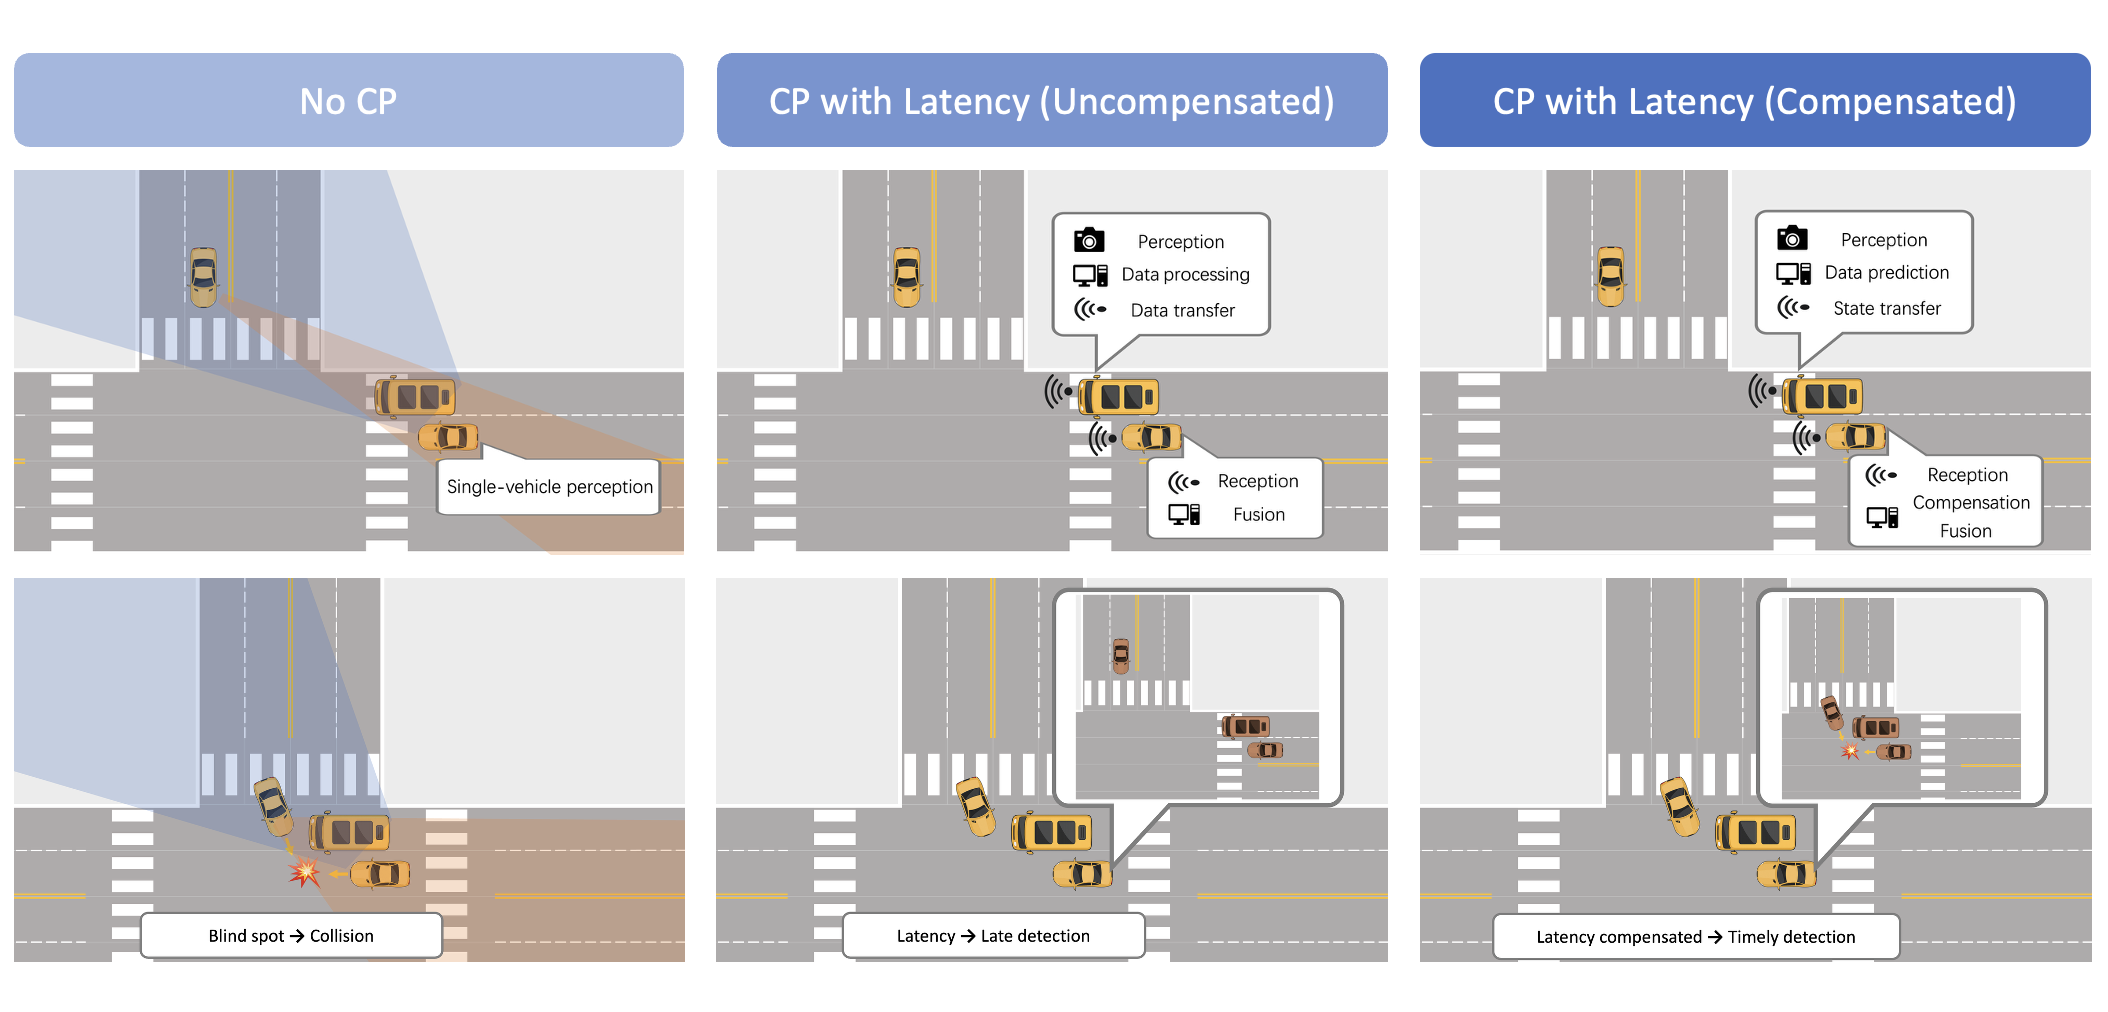
\includegraphics[width=7in]{figure1.jpg}
\caption{\textbf{Example of vehicle perception results under dual-latency.} The figure illustrates three scenarios: \textbf{No CP}, where a single vehicle relies solely on its onboard sensors, resulting in blind spots and potential collisions; \textbf{CP with latency (Uncompensated)}, where cooperative perception is performed but communication and computation latencies cause late detection; and \textbf{CP with latency (Compensated)}, where the proposed mechanism integrates prediction and latency compensation, enabling timely detection and improved real-time performance of perception.
}
\label{fig_1}
\end{figure*}

The main contributions of this paper are summarized as follows:

\begin{enumerate}

\item{Dual-Latency Prediction Compensation Mechanism: We propose a novel compensation mechanism that jointly addresses both communication and computation latencies, ensuring timely and reliable cooperative perception in dynamic traffic environments.}

\item{Vehicle-Specific Prediction Model: Instead of relying on generic models, we design a lightweight prediction model trained on each vehicle’s historical perception data, which enables personalized and more accurate prediction while enhancing robustness against diverse motion patterns.}

\item{Model State Transmission: We introduce an efficient communication strategy that transmits compressed intermediate model states rather than raw perception data. This design not only reduces communication overhead but also offloads redundant computation from the receiver, ensuring efficient resource utilization and sufficient historical context for accurate prediction.}

\item{Enhanced System Performance: By combining personalized prediction, efficient model state transmission, and dual-latency compensation, the proposed mechanism significantly improves the real-time performance, robustness, and adaptability of cooperative perception. Experiments on V2X-Sim and complementary DAIR-V2X-C official detection/BEV forecasting evaluations further validate its effectiveness under simulated and real cooperative driving scenarios.}
\end{enumerate}

\noindent


This paper is organized as follows: Section 2 reviews related work and research background; Section 3 introduces in detail the dual-latency prediction compensation mechanism based on the vehicle-specific Prediction Model proposed in this paper; Section 4 provides experimental setup and result analysis; finally, Section 5 summarizes the paper and looks forward to future research directions.


\noindent
\section{Related Work}
Cooperative perception (CP) enhances environmental awareness by enabling vehicles to share and fuse perception beyond the limits of single-vehicle sensors. Despite these advances, the end-to-end real-time performance of CP remains constrained by latency caused by both communication and computation. Prior studies can be broadly categorized into two research threads: communication latency mitigation and computation latency mitigation. Representative approaches within each thread are reviewed, highlighting their core ideas, mechanisms, and limitations that motivate the proposed method.



% 需要的宏包（导言区）：
% \usepackage{booktabs}
% \usepackage{amssymb}   % 提供 \checkmark
% \usepackage{pifont}    % 提供 -- 作为叉号

\begin{table*}[htbp]
\centering
\caption{Comparison of Existing Approaches and Dual-Latency Prediction Compensation Mechanism (DLPCM)}
\label{related work}
\renewcommand{\arraystretch}{1.3}
\begin{tabular}{@{}l l cc ccc c@{}}
\toprule
\textbf{Reference} & \textbf{Approach}
& \multicolumn{2}{c}{\textbf{\shortstack{Proactive reduction\\of communication overhead}}}
& \multicolumn{3}{c}{\textbf{\shortstack{Reactive mitigation\\of communication impact}}}
& \textbf{\shortstack{Considering\\computation latency}} \\
\cmidrule(lr){3-4} \cmidrule(lr){5-7}
& &
\textbf{\shortstack{Efficient\\resource\\utilization}} &
\textbf{\shortstack{Reduced\\communication\\overhead}} &
\textbf{\shortstack{Alignment\\or\\compensation}} &
\textbf{\shortstack{Sufficient\\historical\\data}} &
\textbf{\shortstack{Vehicle-specific\\prediction}} &
\\
\midrule
\cite{xu2022opv2v,wang2023vimi,zheng2024real,yuan2022keypoints,lohdefink2020focussing,hu2022where2comm}
& Data compression / ROI selection
& \checkmark & \checkmark & -- & -- & -- & -- \\
\cite{liu2020who2com,qu2024model}
& Communication partner selection
& \checkmark & \checkmark & -- & -- & -- & -- \\
\cite{liu2024select2col,liu2024v2x,lin2024v2vformer,lei2024robust,bai2023vinet}
& Temporal alignment
& -- & -- & \checkmark & -- & -- & -- \\
\cite{wang2025cmp,rossle2024unlocking,fang2024pacp,yu2023vehicle,lei2022latency}
& Prediction-based compensation
& -- & -- & \checkmark & -- & -- & -- \\
\midrule
Ours
& DLPCM based on VSPM
& \checkmark & \checkmark & \checkmark & \checkmark & \checkmark & \checkmark \\
\bottomrule
\end{tabular}
\end{table*}




\subsection{Communication Latency Mitigation}
Existing methods for communication latency mitigation can be classified into four main categories: \emph{reducing per-transmission data volume}, \emph{reducing communication links}, \emph{temporal alignment}, and \emph{prediction-based compensation}.

(i) Reducing per-transmission data volume.  
One representative approach minimizes the payload size per communication cycle by compressing raw perception data or feature-level data~\cite{xu2022opv2v,wang2023vimi,zheng2024real}. Alternatively, some methods focus on transmitting only regions of interest (ROI) selected based on saliency or task relevance~\cite{yuan2022keypoints,lohdefink2020focussing,hu2022where2comm}. Although these strategies effectively reduce bandwidth usage and communication overhead, data exchange is still required, meaning latency cannot be fully avoided. Moreover, ROI-based selection risks omitting important contextual information that may be crucial for accurate perception.

(ii) Reducing communication links.  
Another research direction minimizes redundant data transmissions by optimizing communication partner selection~\cite{liu2020who2com,qu2024model}. By choosing only the most informative peers, these methods improve communication efficiency and reduce the communication load across communication links. However, fewer communication links may lead to information loss, particularly in scenarios where excluded vehicles observe unique environmental details. Additionally, latency on the remaining links still persists.

(iii) Temporal alignment.  
To address asynchrony in received information, several studies align delayed perception data with the receiver’s local timeline before fusion~\cite{liu2024select2col,liu2024v2x,lin2024v2vformer,lei2024robust,bai2023vinet}. Such temporal synchronization ensures consistency between onboard and remote observations, improving fusion quality. However, these techniques may inadvertently propagate abnormal or corrupted data forward, potentially compromising system safety in critical situations.

(iv) Prediction-based compensation.  
Instead of merely aligning delayed information, prediction-based approaches attempt to compensate for latency by forecasting the current state of the transmitting vehicle using its historical data~\cite{wang2025cmp,rossle2024unlocking,fang2024pacp,yu2023vehicle,lei2022latency}. These methods can reduce the effective latency and improve fusion accuracy. However, prediction-based compensation suffers from three key limitations: (1) it fails during initial transmissions when no historical data are available, (2) most models lack personalization and cannot adapt to vehicle-specific dynamics, and (3) inconsistent communication delays among transmitting vehicles lead to a substantial increase in the computational load on the receiving vehicle.








\subsection{Computation Latency Mitigation}
Computation latency arises from the limited processing capacity of onboard systems and the computational complexity of perception algorithms. Existing studies tackle this issue through three main strategies: \emph{resource scheduling and parallelization}, \emph{hardware acceleration}, and \emph{algorithmic optimization}.

(i) Resource scheduling and parallelization.  
Systems-oriented approaches aim to better exploit computing resources by parallelizing perception tasks and optimally distributing workloads across heterogeneous processors~\cite{xu2024intelligent,lu2025joint}. These strategies significantly improve processing efficiency and shorten response times. However, since perception tasks inherently involve complex computations, residual latency persists, and outputs may still lag behind the real-time dynamics of the driving environment.

(ii) Hardware acceleration. 
Some studies enhance computational throughput using dedicated hardware accelerators equipped with composable processing units and hierarchical instruction sets~\cite{fan2023hardware}. While such designs improve raw processing speed and system scalability. It often fails to achieve strict real-time guarantees, particularly when perception pipelines become increasingly deep and multi-modal.

(iii) Algorithmic optimization.
A complementary direction focuses on improving algorithmic efficiency by redesigning model architectures. For example, the Informer model~\cite{zhou2021informer} leverages a transformer-based architecture optimized for long-sequence modeling, significantly reducing computational cost while maintaining performance. Nonetheless, such optimizations are often task-specific and fail to generalize across diverse CP workloads, leaving substantial computation latency unaddressed.


In summary, existing efforts on communication latency mitigation reduce payloads, prune redundant links, align delayed information, or compensate for delays via prediction. However, these strategies either retain unavoidable communication latency, risk propagating abnormal data, or lack personalization and fail in initial transmission scenarios. Similarly, computation latency mitigation through resource scheduling, hardware acceleration, and algorithmic optimization reduces but does not eliminate processing delays, leading to residual perception latency. These limitations highlight the need for a unified solution that jointly compensates for both communication and computation latencies, leverages vehicle-specific historical information for personalized prediction, and ensures real-time reliability under dynamic driving conditions. A detailed comparison of related approaches is provided in Table~\ref{related work}.





% \section{Related Work}
% Recent advances in CP have significantly improved environmental awareness by enabling vehicles to share and fuse perception data beyond the limits of single-vehicle onboard sensors. However, the real-time performance of CP is still constrained by latency that occur during communication and computation. As a result, existing studies have primarily concentrated on two aspects: communication latency mitigation and computation latency mitigation. In the following, representative approaches are discussed within these two categories, with a focus on summarizing their key ideas and limitations and highlighting the motivation for our proposed method.
% \subsection{Communication Latency Mitigation}
% Representative approaches for mitigating communication latency in CP are summarized in Table~\ref{tab:comm_latency}. Existing studies can be broadly classified into four categories: (i) reducing the data volume per transmission, (ii) reducing communication links, (iii) temporal alignment, and (iv) prediction-based compensation.



% \begin{table*}[t]
% \centering
% \caption{Representative methods for communication latency mitigation in cooperative perception.}
% \label{tab:comm_latency}
% \small
% \renewcommand{\arraystretch}{1.21}
% \begin{tabularx}{\textwidth}{@{}>{\raggedright\arraybackslash}p{2cm} >{\raggedright\arraybackslash}p{3cm} Y Y@{}}
% \toprule
% \makecell[l]{\textbf{Method}} &
% \makecell[l]{\textbf{Idea}} &
% \makecell[l]{\textbf{Specific Approach}} &
% \makecell[l]{\textbf{Limitation}} \\
% \midrule
% ~\cite{xu2022opv2v,wang2023vimi,zheng2024real,yuan2022keypoints,lohdefink2020focussing,hu2022where2comm} &
% Reduce data volume per transmission &
% Compress perception data to reduce transmission size / ROI-focused transmission &
% Communication latency still remains; risk of missing important data \\
% \addlinespace[2pt]
% ~\cite{liu2020who2com,qu2024model} &
% Reduce communication links &
% Communication partner selection to minimize redundant transmissions &
% Potential information loss; latency cannot be fully avoided \\
% \addlinespace[2pt]
% ~\cite{liu2024select2col,liu2024v2x,lin2024v2vformer,lei2024robust,bai2023vinet} &
% Temporal alignment &
% Synchronize received information to the receiver’s local timeline &
% Risk of propagating abnormal data, compromising safety \\
% \addlinespace[2pt]
% ~\cite{wang2025cmp,rossle2024unlocking,fang2024pacp,yu2023vehicle,lei2022latency} &
% Prediction-based compensation &
% Receiver-side generic models use historical data to predict current state &
% Fail in initial transmission (no history); lack personalization; limited accuracy \\
% \bottomrule
% \end{tabularx}
% \end{table*}





% The first category focuses on reducing the data volume per transmission. Typical methods compress raw perception data~\cite{xu2022opv2v,wang2023vimi,zheng2024real} or select salient regions of interest (ROI)~\cite{yuan2022keypoints,lohdefink2020focussing,hu2022where2comm}, thereby lowering communication overhead. While these strategies effectively reduce bandwidth consumption, perception data must still be exchanged, and communication latency remains unavoidable.

% The second category aims to reduce communication links. By selectively choosing communication partners~\cite{liu2020who2com,qu2024model}, these methods minimize redundant transmissions and improve efficiency. However, the reduced communication links may lead to information loss, and latency cannot be eliminated.

% The third category addresses latency through temporal alignment. Studies such as~\cite{liu2024select2col,liu2024v2x,lin2024v2vformer,lei2024robust,bai2023vinet} synchronize received information with the receiver’s local perception timeline. This ensures temporal consistency between transmitted and local data, but risks propagating abnormal information, which may compromise safety.

% The fourth category employs prediction-based compensation. The models on receiving vehicle~\cite{wang2025cmp,rossle2024unlocking,fang2024pacp,yu2023vehicle,lei2022latency} leverage historical data from the transmitting vehicle to predict its current perception, thereby mitigating the effect of latency. However, these generic models often lack personalization, may fail during the initial transmission when historical data are unavailable, and cannot capture vehicle-specific perception characteristics.






% \subsection{Computation Latency Mitigation}
% Representative methods for mitigating computation latency in cooperative perception are summarized in Table~\ref{tab:comp_latency}. Existing studies can be broadly divided into three categories: (i) computational resource scheduling optimization, (ii) enhancing computational capability through hardware acceleration, and (iii) algorithmic optimization to reduce computation latency.


% \begin{table*}[t]
% \centering
% \caption{Representative methods for computation latency mitigation in cooperative perception.}
% \label{tab:comp_latency}
% \small
% \renewcommand{\arraystretch}{1.21}
% \begin{tabularx}{\textwidth}{@{}>{\raggedright\arraybackslash}p{2cm} >{\raggedright\arraybackslash}p{3cm} Y Y@{}}
% \toprule
% \makecell[l]{\textbf{Method}} &
% \makecell[l]{\textbf{Idea}} &
% \makecell[l]{\textbf{Specific Approach}} &
% \makecell[l]{\textbf{Limitation}} \\
% \midrule
% ~\cite{xu2024intelligent,lu2025joint} &
% Computational resource scheduling optimization &
% Parallelization and optimized allocation of perception tasks across computing units &
% Latency reduced but not eliminated; outputs may still lag behind dynamic environments \\
% \addlinespace[2pt]
% ~\cite{fan2023hardware} &
% Enhance computational capability &
% Custom accelerator with composable units and hierarchical instruction set &
% Real-time performance not fully achieved \\
% \addlinespace[2pt]
% ~\cite{zhou2021informer} &
% Algorithmic optimization &
% Algorithmic optimization with efficient sequence modeling to reduce latency &
% Task-specific; cannot fully eliminate computation latency \\
% \bottomrule
% \end{tabularx}
% \end{table*}




% The first category focuses on resource scheduling optimization. Methods such as~\cite{xu2024intelligent,lu2025joint} improve efficiency by parallelizing computation and optimizing the allocation of tasks across available processing units. These approaches can significantly shorten processing time, yet perception results may still lag behind real-world traffic state, and real-time responsiveness is not fully guaranteed.

% The second category enhances computational capability through hardware acceleration. Representative study optimizes accelerator with composable units and hierarchical instruction set~\cite{fan2023hardware}. While these solutions improve hardware processing speed, they cannot completely eliminate computation latency.

% The third category emphasizes algorithmic optimization. For instance, the Informer model~\cite{zhou2021informer} introduces an efficient transformer architecture, demonstrating the potential to reduce computation latency by improving algorithmic efficiency. However, such models are often tailored for specific scenario, and cannot fully eliminate computation latency.

% In summary, existing works provide valuable foundations for addressing latency issues in cooperative perception. Communication latency mitigation has focused on reducing transmission overhead, synchronizing delayed data, or compensating latency through prediction models, yet these methods either fail to eliminate latency, risk propagating abnormal information, or lack vehicle-specific adaptation. Computation latency mitigation has leveraged resource scheduling optimization, hardware acceleration and algorithmic optimization, but the problem of perception computation latency persists. These limitations underline the need for a more comprehensive solution that can jointly compensate for both communication and computation latencies, while also leveraging vehicle-specific historical information to improve prediction accuracy and ensure real-time reliability.

















 

\section{Dual-latency Prediction Compensation Mechanism Based on the Vehicle-Specific Prediction Model}
\label{sec:method}






\begin{figure*}[!t]
\centering
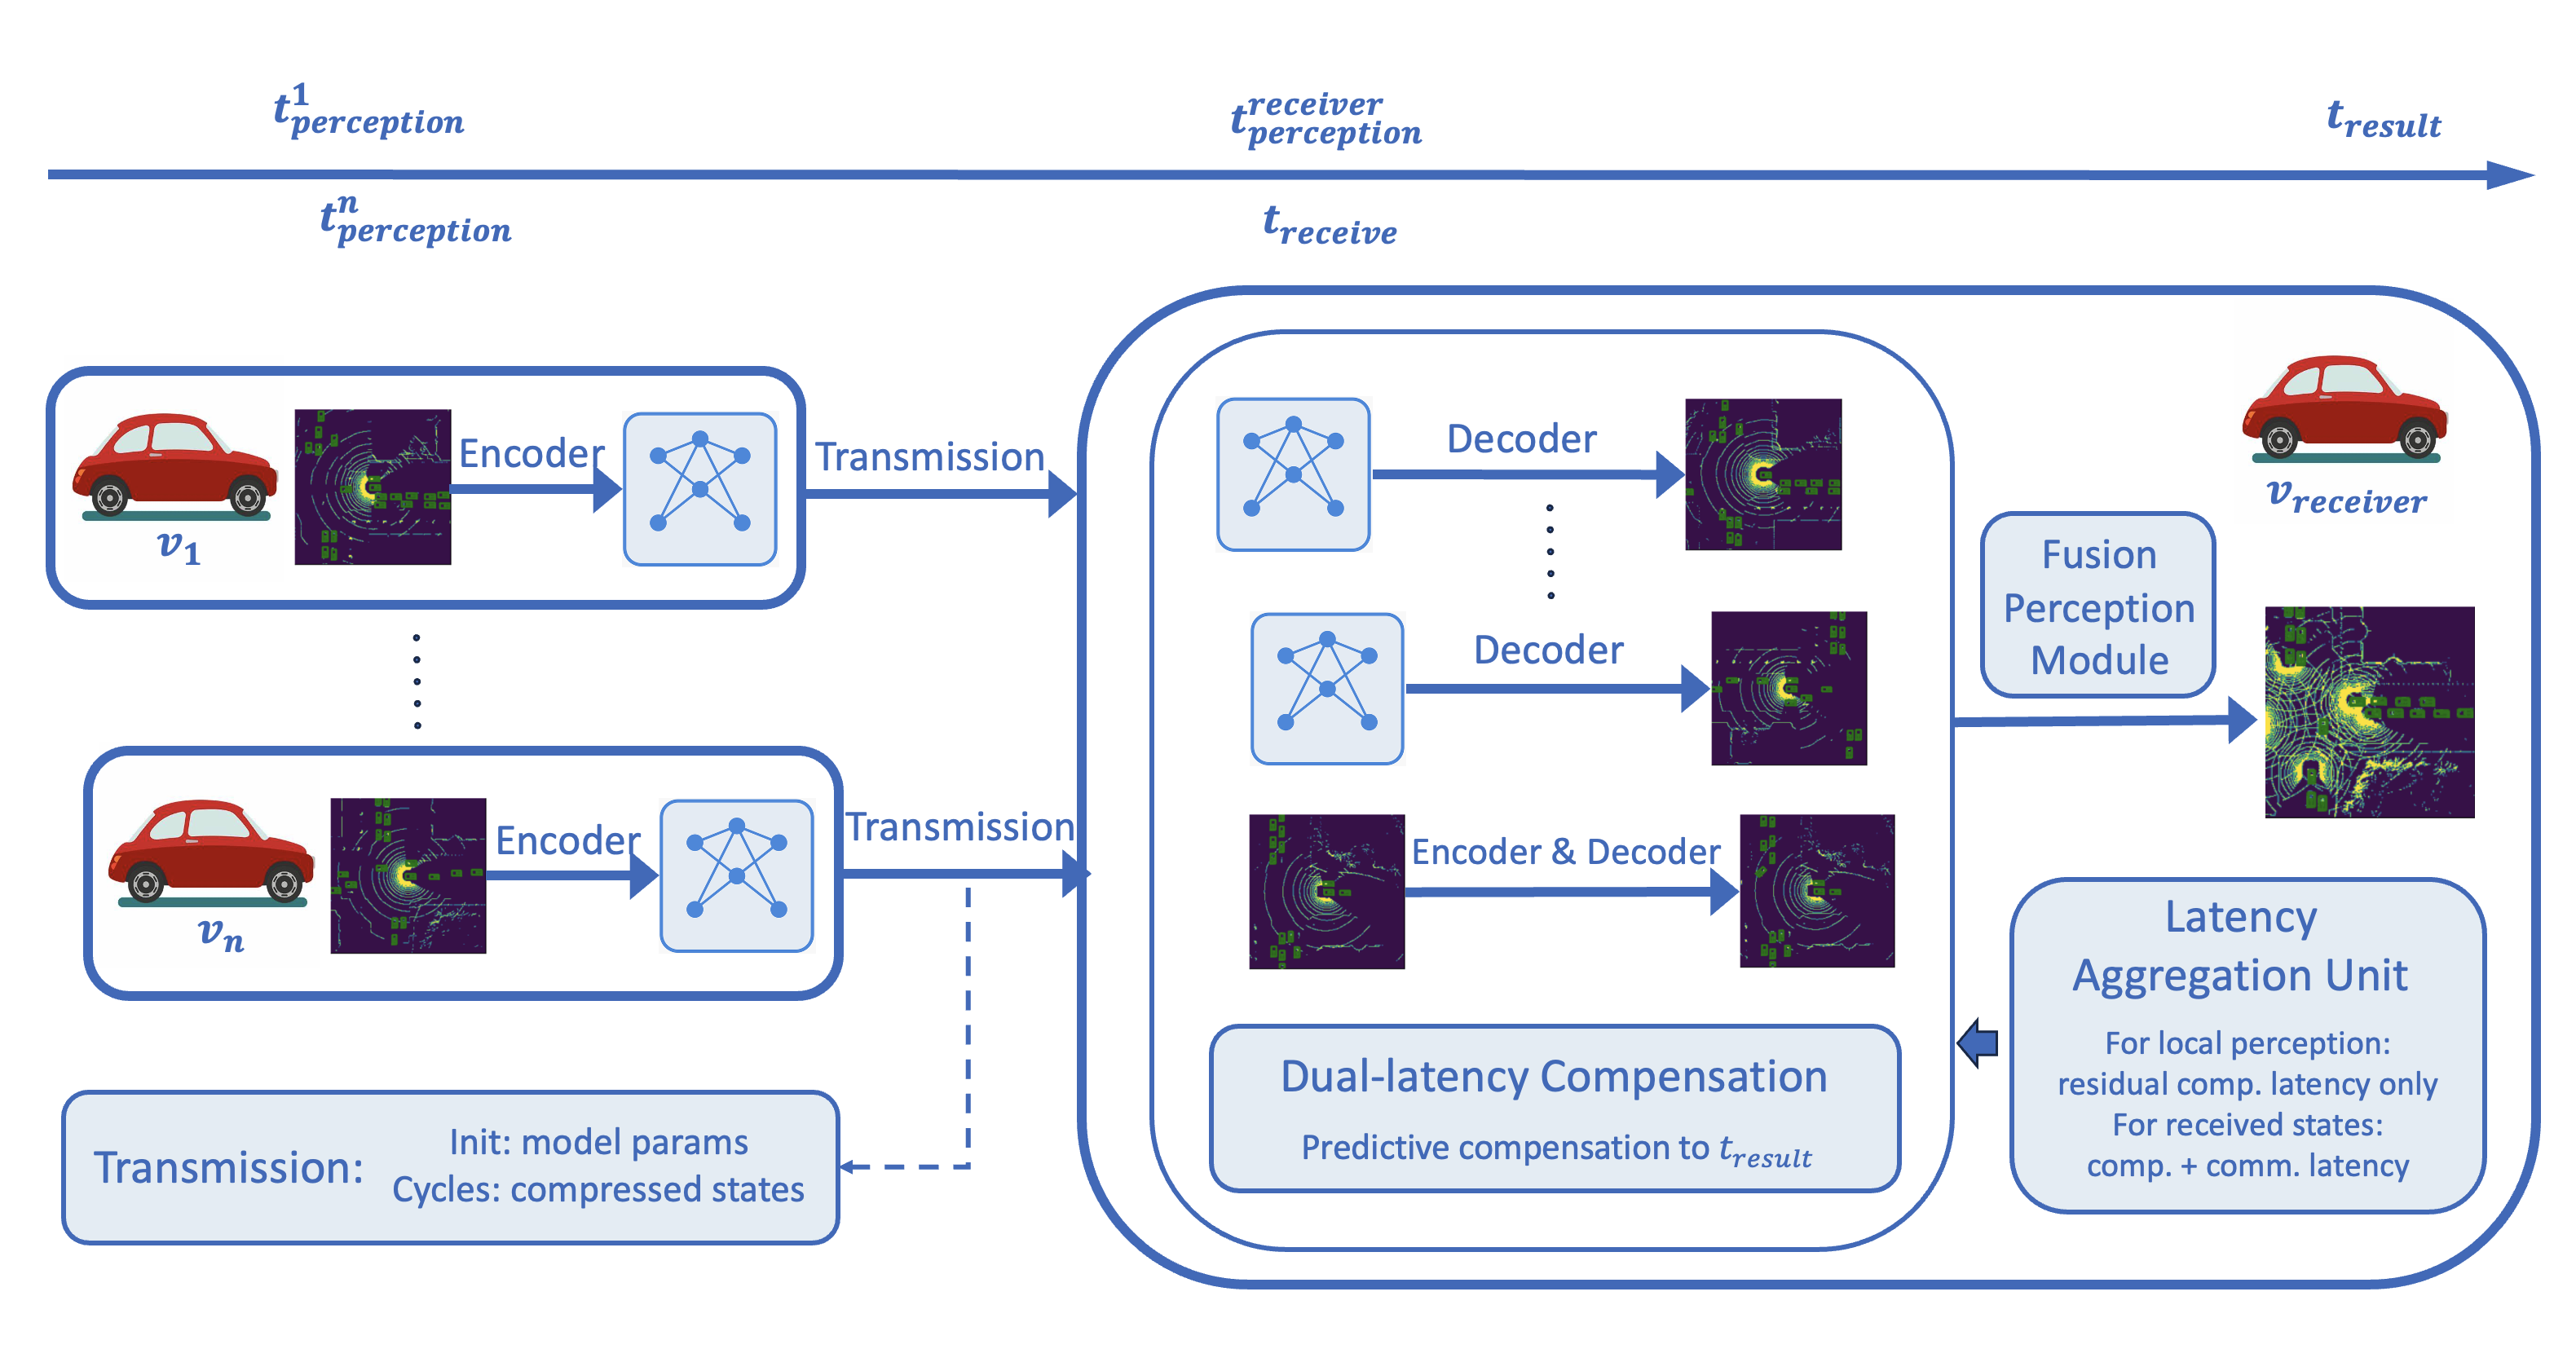
\includegraphics[width=7in]{figure2.png}
\caption{\textbf{Framework of dual-latency prediction compensation mechanism based on the
transmitter model.} 
$t^{n}_{perception}$ denotes the perception time of the $n$-th transmitting vehicle; 
    $t_{receive}$ is the time when the receiver obtains the last transmitted state; 
    $t^{receiver}_{perception}$ indicates the receiver’s latest local perception time, which coincides with $t_{receive}$; 
    and $t_{result}$ represents the expected time when computation is completed and the final perception result is obtained. 
\\Each transmitting vehicle encodes its local perception and \textbf{transmits either }\textbf{model parameters (initial exchange) or compressed intermediate states (subsequent cycles)}. Upon reception, each transmitted state is decoded using the corresponding vehicle’s prediction model, and then compensated to $t_{result}$ by accounting for \textbf{both communication and computation latencies}. Simultaneously, when the last state is received, the receiver obtains its latest local perception at $t^{receiver}_{perception} = t_{receive}$, which is further compensated for the residual computation latency to reach $t_{result}$. Finally, all latency-compensated data are synchronized at $t_{result}$ and fused within the fusion perception module, yielding timely environmental awareness.}
\label{fig_2}
\end{figure*}




In this section, we present a cooperative perception framework that addresses both \emph{communication latency} and \emph{computation latency} through a \emph{Dual-Latency Prediction Compensation Mechanism} as shown in Figure~\ref{fig_2}. The proposed approach is built upon a \emph{Vehicle-Specific Prediction Model} deployed at the transmitting vehicle and an efficient \emph{Model State Transmission} protocol, enabling the receiver to reconstruct the transmitter's future perception results and perform latency-compensated fusion. The proposed mechanism significantly enhances the real-time performance and robustness of cooperative perception. The overall procedure of the proposed mechanism is summarized in Algorithm~\ref{alg:dual_latency}.






\subsection{Vehicle-Specific Prediction Model}
\label{subsec:vspm}

To exploit the transmitter’s rich vehicle-specific history while minimizing communication cost and receiver-side latency, we instantiate $\mathcal{M}_{\theta_i}$ as a lightweight encoder--decoder ConvLSTM trained offline on vehicle $i$’s logs. The model learns idiosyncratic motion and sensing patterns from historical data and exposes compact decoder states $(\mathbf{h}^i_t,\mathbf{c}^i_t)$ that align with the state-transmission interface in \S\ref{subsec:state} and the dual-latency compensation in \S\ref{subsec:fusion}. The perception representation is a binary bird’s-eye-view (BEV) occupancy grid, denoted as $X^i_t \in \{0,1\}^{H\times W}$. Unless otherwise specified, $X^i_t$ also serves as the training supervision $Y^i_t$.

\subsubsection{Model architecture}
We realize the temporal transition $f_{\theta_i}$ (cf.\ Eq.~\ref{eq:lstm_update}) with a single-layer ConvLSTM using $3{\times}3$ convolutions (unit padding) and hidden width $32$. 
An \emph{encoder} ConvLSTM consumes the history $\mathcal{X}^i_{1:T}=\{X^i_1,\dots,X^i_T\}$ and summarizes it into $(\mathbf{h}^i_T,\mathbf{c}^i_T)$, 
where $\mathbf{h}^i_T$ denotes the final hidden state capturing spatial-temporal features, and $\mathbf{c}^i_T$ is the cell state that preserves long-term temporal memory.
A matched \emph{decoder} ConvLSTM, initialized with $(\mathbf{h}^i_T,\mathbf{c}^i_T)$, rolls the state forward for $S$ horizons. 
During \emph{training at the transmitter}, the first decoder input is the last observed frame and subsequent inputs follow the scheduled-sampling policy described below (see \S\ref{subsec:vspm} ``Autoregressive decoding''). 
Readout $g_{\theta_i}$ is implemented by a lightweight occupancy head,
\emph{Conv}$(32{\to}32,\,3{\times}3)$ + ReLU followed by \emph{Conv}$(32{\to}1,\,1{\times}1)$ and a sigmoid,
which maps decoder states to calibrated per-pixel probabilities $\widehat{Y}^i_k \in [0,1]^{H\times W}$.
We keep the decoder’s states compact so that the \emph{compressed intermediate model states} $(\mathbf{h}^i_t,\mathbf{c}^i_t)$ can serve as a transmissible state payload in $\mathcal{P}^{i\rightarrow j}$ with negligible bandwidth.

\subsubsection{Transmissible state and rollout interface}
The decoder’s \emph{compressed intermediate model states} $(\mathbf{h}^i_s,\mathbf{c}^i_s)$, 
representing the hidden and cell states of the ConvLSTM, 
serve as the compact predictive state. 
Given the transmitted states at sender time $s$, the receiver uses the cached $\theta_i$ and a rollout operator $\mathcal{R}(\cdot,\cdot,\widehat{\Delta})$ 
to advance the states and decode the transmitter’s occupancy prediction at the receiver’s current time:
\begin{equation}
\begin{aligned}
(\mathbf{h}',\mathbf{c}') \;=\; \mathcal{R}\!\big((\mathbf{h}^i_s,\mathbf{c}^i_s),\,\widehat{\Delta}\big), 
\qquad
\widehat{Y}^{i\rightarrow j}_{t} \;=\; g_{\theta_i}(\mathbf{h}').
\end{aligned}
\label{eq:state_update_and_prediction}
\end{equation}

Here, $\mathcal{R}$ corresponds to an \emph{autoregressive ConvLSTM transition}: at each rollout step,
\begin{equation}
(\mathbf{h}_{s+k},\mathbf{c}_{s+k}) = f_{\theta_i}\!\big(\mathbf{h}_{s+k-1},\mathbf{c}_{s+k-1}\big),
\label{eq:lstm_update}
\end{equation}

reusing the decoder’s own predicted occupancy from the previous step instead of any ground-truth inputs.
On the receiver, $\mathcal{R}$ runs in \emph{free mode without external inputs}, 
i.e., no raw frame $X^i_s$ is required in the packet.

$\widehat{\Delta}$ aggregates communication and computation latencies as defined in \S\ref{subsec:fusion}. 
For implementation convenience in our experiments, we quantize sequences with a temporal step $\Delta\tau=0.2\,$s and advance $\mathcal{R}$ by the corresponding number of discrete steps.

\subsubsection{Autoregressive decoding (training-time)}
Decoding is autoregressive. To mitigate exposure bias, we employ scheduled sampling: early epochs feed ground-truth previous frames to the decoder, and the policy smoothly transitions to self-feeding predictions as training progresses. Validation and test always run in free mode (self-feeding only) to reflect deployment behavior (which matches the receiver-side rollout described above).







\subsubsection{Training objectives}

\paragraph{Per-pixel dynamic weights}
For each pixel $(u,v)$, we define the dynamic mask and weights as:
\begin{align}
D^i_k(u,v) &= \mathbf{1}\!\left(X^{i,\mathrm{prev}}_k(u,v) \neq Y^i_k(u,v)\right), \\
w^i_k(u,v) &= 1 + \lambda_d\, D^i_k(u,v),
\label{eq:dynmask_weights_pixel}
\end{align}
where $X^{i,\mathrm{prev}}_k$ is the previous-frame input to the decoder at step $k$, and $\lambda_d \ge 0$ controls the emphasis on dynamic pixels. Setting $\lambda_d=0$ reduces to uniform weighting. During training with scheduled sampling,
$X^{i,\mathrm{prev}}_k \;=\; \alpha_k\,Y^i_{k-1} + (1-\alpha_k)\,\widehat{Y}^i_{k-1},$
where $\alpha_k\in\{0,1\}$ follows the schedule.
This weighting scheme highlights regions with motion changes, improving predictive performance on dynamic objects.

\paragraph{Dynamic binary cross-entropy (BCE)}
The BCE loss measures per-pixel occupancy prediction fidelity, enhanced with dynamic motion-aware weighting:
\begin{align}
&\mathrm{BCE}(\widehat{Y}^i_k, Y^i_k;\, w^i_k)
= - \frac{1}{HW} \sum_{u=1}^{H} \sum_{v=1}^{W} w^i_k(u,v) \notag \\
&\qquad \times \Bigl[
    Y^i_k(u,v) \cdot \log \widehat{Y}^i_k(u,v) \notag \\
&\quad + \big(1-Y^i_k(u,v)\big) \cdot \log \big(1-\widehat{Y}^i_k(u,v)\big)
\Bigr].
\label{eq:bce_loss}
\end{align}

\paragraph{Dice loss}
To address class imbalance in sparse occupancy grids, we employ the Dice coefficient loss:
\begin{align}
\mathrm{Dice}(\widehat{Y}^i_k, Y^i_k)
= 1 - \frac{2 \sum\limits_{u,v} \widehat{Y}^i_k(u,v) \, Y^i_k(u,v) + \epsilon}
              {\sum\limits_{u,v} \widehat{Y}^i_k(u,v) + \sum\limits_{u,v} Y^i_k(u,v) + \epsilon},
\label{eq:dice_loss}
\end{align}
where $\epsilon$ is a small constant ($10^{-6}$) for numerical stability. The Dice loss directly optimizes the overlap between predicted and true occupancy masks, especially benefiting underrepresented dynamic regions.

\paragraph{Curriculum warmup for auxiliary losses}  
To stabilize the early stage of training, we adopt a curriculum warmup strategy for the Dice loss only. Let $e$ denote the current training epoch (starting from $1$). During the initial $E_{\mathrm{warm}}$ epochs, we optimize only the dynamic-weighted BCE loss defined in Eq.~\eqref{eq:bce_loss}. After the warmup stage, the Dice loss term is gradually introduced over an additional $E_{\mathrm{ramp}}$ epochs by increasing its coefficient with a compact schedule:
\[
\lambda_{\mathrm{dice}}(e) \;=\; \lambda_{\mathrm{dice}}^\ast \cdot \min\!\Bigl\{1,\;\max\!\bigl\{0,\;\tfrac{e-E_{\mathrm{warm}}}{E_{\mathrm{ramp}}}\bigr\}\Bigr\}.
\]
Beyond $E_{\mathrm{warm}} + E_{\mathrm{ramp}}$ epochs, the Dice weight remains fixed at $\lambda_{\mathrm{dice}}^\ast$.

\paragraph{Training loss}
Our final per-step training loss is defined as:
\begin{align}
\mathcal{L}^i_k
&=\;
\underbrace{\mathrm{BCE}\!\left(\widehat{Y}^i_k, Y^i_k; w^i_k\right)}_{\text{occupancy prediction}}
\;+\;
\lambda_{\mathrm{dice}}(e)\,
\mathrm{Dice}\!\left(\widehat{Y}^i_k, Y^i_k\right).
\label{eq:final_loss}
\end{align}
The sequence-level objective averages the horizon-wise losses:
\[
\mathcal{L}^i = \frac{1}{S}\sum_{k=1}^{S}\mathcal{L}^i_k.
\]

\subsubsection{Training protocol}
We optimize with AdamW (learning rate $10^{-3}$), batch size $8$, for $30$ epochs. Data augmentation applies horizontal flips and $180^\circ$ rotations with probability $0.5$ to both history and targets. Inputs are rasterized from sparse $(y,x)$ indices into $H{\times}W$ binary grids (default $256{\times}256$). Encoder/decoder ConvLSTMs use hidden width $32$ and $3{\times}3$ kernels; validation is logged per horizon in free-running mode.
%In deployment, the transmitter runs the encoder/decoder online, transmits the \emph{compressed intermediate model states} $(\mathbf{h}^i_t,\mathbf{c}^i_t)$ (with timestamp and pose) as the compact state, and the receiver reconstructs $\widehat{Y}^i_{t}$ via Eq.~\eqref{eq:vspm_rollout_interface} using horizon $\widehat{\Delta}$, ensuring consistency with the dual-latency compensation pipeline in \S\ref{subsec:fusion}.






\subsection{Model State Transmission}
\label{subsec:state}

\subsubsection{One-Time Model Parameter Transmission}
During the initial vehicle-to-vehicle (V2V) communication, vehicle $i$ transmits its trained model parameters $\theta_i$ to the receiver. These parameters are sent only once and reused for all subsequent interactions, avoiding repeated transmission of large model parameters or feature tensors.

\subsubsection{Lightweight State Updates}
In subsequent communication cycles, the transmitting vehicle \(i\) no longer sends raw perception data or high-dimensional feature maps to the receiving vehicle \(j\). 
Instead, it transmits only the \emph{compressed intermediate model states}, defined as the decoder’s hidden and cell states \((\mathbf{h}^i_{t_{\text{per}}},\mathbf{c}^i_{t_{\text{per}}})\), along with the sender perception timestamp and pose:
\begin{equation}
    \mathcal{P}^{i \rightarrow j}(t_{\text{per}}\!\to\!t) 
    = \{\mathbf{h}^i_{t_{\text{per}}}, \mathbf{c}^i_{t_{\text{per}}}, t_{\text{per}}, \mathbf{T}^i_{t_{\text{per}}}\},
\end{equation}
where \(\mathbf{h}^i_{t_{\text{per}}}\) and \(\mathbf{c}^i_{t_{\text{per}}}\) are the decoder’s hidden and cell states at the sender's perception time \(t_{\text{per}}\), 
\(\mathbf{T}^i_{t_{\text{per}}}\) is the sender’s ego pose at the same moment, and \(t\) denotes the receiver time when the packet is received.
Here, \(t_{\text{per}}\) specifically indicates the timestamp when the transmitting vehicle \(i\) perceived the input data used to compute the transmitted states.
We refer to \((\mathbf{h}^i_{t_{\text{per}}},\mathbf{c}^i_{t_{\text{per}}})\) collectively as the \emph{compressed intermediate model states} since they provide a compact yet sufficient representation for prediction continuation. 
This design greatly reduces bandwidth usage while preserving the information necessary for accurate future prediction on the receiver side. 

% \paragraph{Advantages of Sending Compressed Intermediate States}
% Sending \emph{compressed intermediate model states} instead of raw perception data provides three main benefits:

% \begin{itemize}
%     \item \textbf{Efficient Computation:}  
%     If the sender transmits raw data, each receiver must independently complete the full prediction, causing redundant computation.  
%     By letting the sender perform most of the prediction process and sharing only intermediate states, receivers only compute the remaining latency-compensation steps, reducing overall computational load.

%     \item \textbf{Better Prediction with Less Data:}  
%     Intermediate states already encode sufficient historical context.  
%     This avoids the need to transmit large volumes of past sensor data while still enabling receivers to achieve accurate predictions, even during the first-time communication.

%     \item \textbf{Lower Communication Overhead:}  
%     Compared to raw frames or high-dimensional features, compressed states are much smaller, significantly reducing bandwidth usage while preserving essential temporal information.
% \end{itemize}






\begin{algorithm}[t]
\caption{Dual-latency Prediction Compensation with Vehicle-Specific Prediction Model (VSPM)}
\label{alg:dual_latency}
\begin{algorithmic}[1]

    \Require Transmitting vehicles \ensuremath{\mathcal{V}}, receiver \ensuremath{\mathrm{re}}
    \Require Cached parameters \ensuremath{\{\theta_i\}}, received packets \ensuremath{\{\mathcal{P}^{i\rightarrow\mathrm{re}}\}}
    \Require Local compressed states \ensuremath{(\mathbf{h}^{\mathrm{re}}_{t^{\mathrm{re}}_{\mathrm{per}}}, \mathbf{c}^{\mathrm{re}}_{t^{\mathrm{re}}_{\mathrm{per}}})}
    \Require Local model parameters \ensuremath{\theta_{\mathrm{re}}}, quantization step \ensuremath{\Delta\tau}

    \Ensure Latency-compensated fused occupancy prediction \ensuremath{\widehat{Y}^{\mathrm{re},\mathrm{fused}}_{t_{\mathrm{result}}}}

    \State \textbf{Initialization:} Each transmitting vehicle \ensuremath{i} sends \ensuremath{\theta_i} once; the receiver caches them.

    \State \textbf{Step 1: Packet Reception}
    \State Receive valid compressed packets at \ensuremath{t_{\mathrm{receive}}}:
    \Statex \hspace{\algorithmicindent}%
    \ensuremath{\mathcal{P}^{i\rightarrow\mathrm{re}}
      = \{\mathbf{h}^i_{t^i_{\mathrm{per}}},\; \mathbf{c}^i_{t^i_{\mathrm{per}}},\; t^i_{\mathrm{per}},\; \mathbf{T}^i_{t^i_{\mathrm{per}}}\}}
    \State Define $\mathcal{N}(\mathrm{re}) = \{\, i \in \mathcal{V} \mid \mathrm{re} \text{ receives a packet from } i \,\}$


    \State \textbf{Step 2: Unified Prediction Time}
    \State Compute \ensuremath{t_{\mathrm{result}} = t_{\mathrm{receive}} + \tau^{\mathrm{re}}_{t_{\mathrm{receive}}}}
    % \State Set waiting time \ensuremath{\delta^{\mathrm{wait}} = \max(0,\; t^{\mathrm{re}}_{\mathrm{start}} - t_{\mathrm{receive}})}

    \State \textbf{Step 3: Remote Branch Rollout}
    \ForAll{\ensuremath{i \in \mathcal{N}(\mathrm{re})}}
        \State \ensuremath{\widehat{\Delta}^{(i)} = t_{\mathrm{result}} - t^i_{\mathrm{per}}}
        %+ \delta^{\mathrm{wait}}}
        \State \ensuremath{K^{(i)} = \max\{0,\; \mathrm{round}(\widehat{\Delta}^{(i)}/\Delta\tau)\}}
        \State \ensuremath{(\mathbf{h}',\mathbf{c}') \gets \mathcal{R}\bigl((\mathbf{h}^i_{t^i_{\mathrm{per}}}, \mathbf{c}^i_{t^i_{\mathrm{per}}}),\; K^{(i)}\bigr)}
        \State \ensuremath{\widehat{Y}^{i\rightarrow\mathrm{re}}_{t_{\mathrm{result}}} = g_{\theta_i}(\mathbf{h}')}
    \EndFor

    \State \textbf{Step 4: Local Branch Rollout}
    \State \ensuremath{\widehat{\Delta}_{\mathrm{re}} = t_{\mathrm{result}} - t^{\mathrm{re}}_{\mathrm{per}}}
    \State \ensuremath{K_{\mathrm{re}} = \max\{0,\; \mathrm{round}(\widehat{\Delta}_{\mathrm{re}}/\Delta\tau)\}}
    \State \ensuremath{(\mathbf{h}',\mathbf{c}') \gets \mathcal{R}\bigl((\mathbf{h}^{\mathrm{re}}_{t^{\mathrm{re}}_{\mathrm{per}}}, \mathbf{c}^{\mathrm{re}}_{t^{\mathrm{re}}_{\mathrm{per}}}),\; K_{\mathrm{re}}\bigr)}
    \State \ensuremath{\widehat{Y}^{\mathrm{re}}_{t_{\mathrm{result}}} = g_{\theta_{\mathrm{re}}}(\mathbf{h}')}

    \State \textbf{Step 5: Spatio-Temporal Alignment}
    \ForAll{\ensuremath{i \in \mathcal{N}(\mathrm{re})}}
        \State Transform \ensuremath{\widehat{Y}^{i\rightarrow\mathrm{re}}_{t_{\mathrm{result}}}} into the receiver frame
        \Statex \hspace{\algorithmicindent}using \ensuremath{\mathbf{T}^i_{t^i_{\mathrm{per}}}} and \ensuremath{\mathbf{T}^{\mathrm{re}}_{t_{\mathrm{result}}}}
    \EndFor

    \State \textbf{Step 6: Confidence-Aware Fusion}
    \State $\displaystyle
        \widehat{Y}^{\mathrm{re},\mathrm{fused}}_{t_{\mathrm{result}}}
        = \mathcal{F}\!\Bigl(
            \widehat{Y}^{\mathrm{re}}_{t_{\mathrm{result}}},
            \{\widehat{Y}^{i\rightarrow\mathrm{re}}_{t_{\mathrm{result}}}\}_{i\in\mathcal{N}(\mathrm{re})}
        \Bigr)
    $

    \State \textbf{Step 7: Output and Buffer Update}
    \State Publish \ensuremath{\widehat{Y}^{\mathrm{re},\mathrm{fused}}_{t_{\mathrm{result}}}} and discard outdated packets

\end{algorithmic}
\end{algorithm}











\subsection{Dual-Latency Predictive Compensation Fusion}
\label{subsec:fusion}
\subsubsection{Computation-latency Estimation}
We define, for vehicle $i$ at time $t$, the elapsed runtime required to (i) process all \emph{compressed state packets} currently stored in its receive buffer together with its own local state, and (ii) compute the final \emph{fused} perception result as $\tau^i_t$. This computation time can be estimated from the vehicle's current computing-unit status and the volume of pending tasks; thus, $\tau^i_t$ can be approximated using an empirical formula. 

\subsubsection{Latency-Aware Prediction}
We describe the procedure from the receiver's perspective. Consider a sender $i$ and a receiver vehicle \emph{receiver}. Let $\mathcal{P}^{i \rightarrow \text{re}}(t^{i}_{\text{per}}\!\to\!t_{\text{receive}})$ represent a compressed state packet generated by sender $i$ at perception time $t^{i}_{\text{per}}$ and received by the \emph{receiver} vehicle at time $t_{\text{receive}}$. The receiver aims to produce a prediction aligned with:
\[
t_{\text{result}} \;=\; t_{\text{receive}} \,+\, \tau^{\text{re}}_{t_{\text{receive}}}.
\]
The corresponding total latency-compensation horizon is given by:
\[
\widehat{\Delta} \;=\; t_{\text{result}} \,-\, t^{i}_{\text{per}}.
\]
%If multiple sender vehicles are present or if packets experience additional waiting time in the receiver buffer before being processed, we add this waiting time to the effective horizon. Specifically, if fusion starts at $t^{\text{re}}_{\text{start}} \ge t_{\text{receive}}$, we define $\delta^{\text{wait}} = t^{\text{re}}_{\text{start}} - t_{\text{receive}}$ and update $\widehat{\Delta} \leftarrow \widehat{\Delta} + \delta^{\text{wait}}$ accordingly.

Using the cached model parameters $\theta_i$ and the \emph{compressed intermediate model states} $(\mathbf{h}^i_{t^{i}_{\text{per}}}, \mathbf{c}^i_{t^{i}_{\text{per}}})$ contained in the packet, the receiver rolls the model forward in free mode by $\widehat{\Delta}$ with the rollout operator $\mathcal{R}(\cdot)$ introduced in \S\ref{subsec:vspm}, and decodes the occupancy prediction aligned to $t_{\text{result}}$:
\[
(\mathbf{h}',\mathbf{c}') \;=\; \mathcal{R}\!\Big((\mathbf{h}^i_{t^{i}_{\text{per}}}, \mathbf{c}^i_{t^{i}_{\text{per}}}),\,\widehat{\Delta}\Big), 
\qquad
\widehat{Y}^{i\rightarrow \text{re}}_{t_{\text{result}}} \;=\; g_{\theta_i}(\mathbf{h}').
\]


\subsubsection{Local Latency Compensation}
In parallel, the receiver compensates for its own computation latency by propagating its most recent local perception at time $t^{\text{re}}_{\text{per}}$ forward to the unified prediction time $t_{\text{result}}$. We define the local latency-compensation horizon as:
\[
\widehat{\Delta}_{\text{re}} \;=\; t_{\text{result}} - t^{\text{re}}_{\text{per}}.
\]
Using the cached local model parameters $\theta_{\text{re}}$ and the \emph{compressed intermediate model states} $(\mathbf{h}^{\text{re}}_{t^{\text{re}}_{\text{per}}}, \mathbf{c}^{\text{re}}_{t^{\text{re}}_{\text{per}}})$, the receiver similarly performs free-mode rollout:
\[
(\mathbf{h}',\mathbf{c}') \;=\; \mathcal{R}\!\Big((\mathbf{h}^{\text{re}}_{t^{\text{re}}_{\text{per}}}, \mathbf{c}^{\text{re}}_{t^{\text{re}}_{\text{per}}}),\,\widehat{\Delta}_{\text{re}}\Big), 
\qquad
\widehat{Y}^{\text{re}}_{t_{\text{result}}} \;=\; g_{\theta_{\text{re}}}(\mathbf{h}').
\]
Thus, both the local and remote predictions are aligned to the same global time $t_{\text{result}}$, enabling subsequent spatio-temporal alignment and multi-vehicle fusion.


\subsubsection{Spatio-Temporal Alignment and Fusion}
To integrate multi-vehicle perception, each reconstructed remote prediction $\widehat{Y}^{i \rightarrow \text{re}}_{t_{\text{result}}}$ is transformed into the receiver’s coordinate frame using the sender’s ego pose $\mathbf{T}^i_{t^{i}_{\text{per}}}$ and the receiver’s ego pose $\mathbf{T}^{\text{re}}_{t_{\text{result}}}$.  
Before fusion, both local and remote predictions are temporally aligned at the unified prediction time $t_{\text{result}}$.  
We then apply a confidence-aware spatio-temporal fusion strategy that combines the compensated local prediction $\widehat{Y}^{\text{re}}_{t_{\text{result}}}$ with all latency-compensated remote predictions:
\begin{equation}
    \widehat{Y}^{\text{re},\mathrm{fused}}_{t_{\text{result}}}
    = \mathcal{F}\!\Big(
        \widehat{Y}^{\text{re}}_{t_{\text{result}}},\,
        \{\widehat{Y}^{i \rightarrow \text{re}}_{t_{\text{result}}}\}_{i \in \mathcal{N}(\text{re})}
    \Big),
\end{equation}
where $\mathcal{F}(\cdot)$ denotes a generic perception fusion operator, providing flexibility to integrate any fusion model.  
Here, $\mathcal{N}(\text{re})$ represents the set of all transmitting vehicles from which the receiver \text{re} has successfully received valid compressed state packets during the current fusion cycle.  
In our experiments, we instantiate $\mathcal{F}$ with V2VNet\cite{wang2020v2vnet} and DiscoNet\cite{li2021learning} fusion head adapted to operate on occupancy probabilities; other strategies can also be seamlessly integrated.


% \subsection{Dual-Latency Compensation and Confidence-Aware Fusion}

% The overall procedure of the proposed Dual-latency Prediction Compensation with Vehicle-Specific Prediction Model (VSPM) is summarized in Algorithm~\ref{alg:dual_latency}. The algorithm first initializes cached vehicle-specific parameters and receives compressed packets from neighboring vehicles. Then, a unified prediction time is determined to synchronize local and remote predictions. For each received packet, the remote branch performs latent state rollout to compensate for communication and processing latencies, while the local branch predicts its own occupancy at the same unified time. Afterward, all remote predictions are transformed into the receiver’s coordinate frame, and a confidence-aware spatio-temporal fusion strategy integrates both local and remote results to produce the final latency-compensated fused occupancy prediction.


\section{Performance Evaluation}

% Figure reference
\begin{figure}[t]
    \centering
    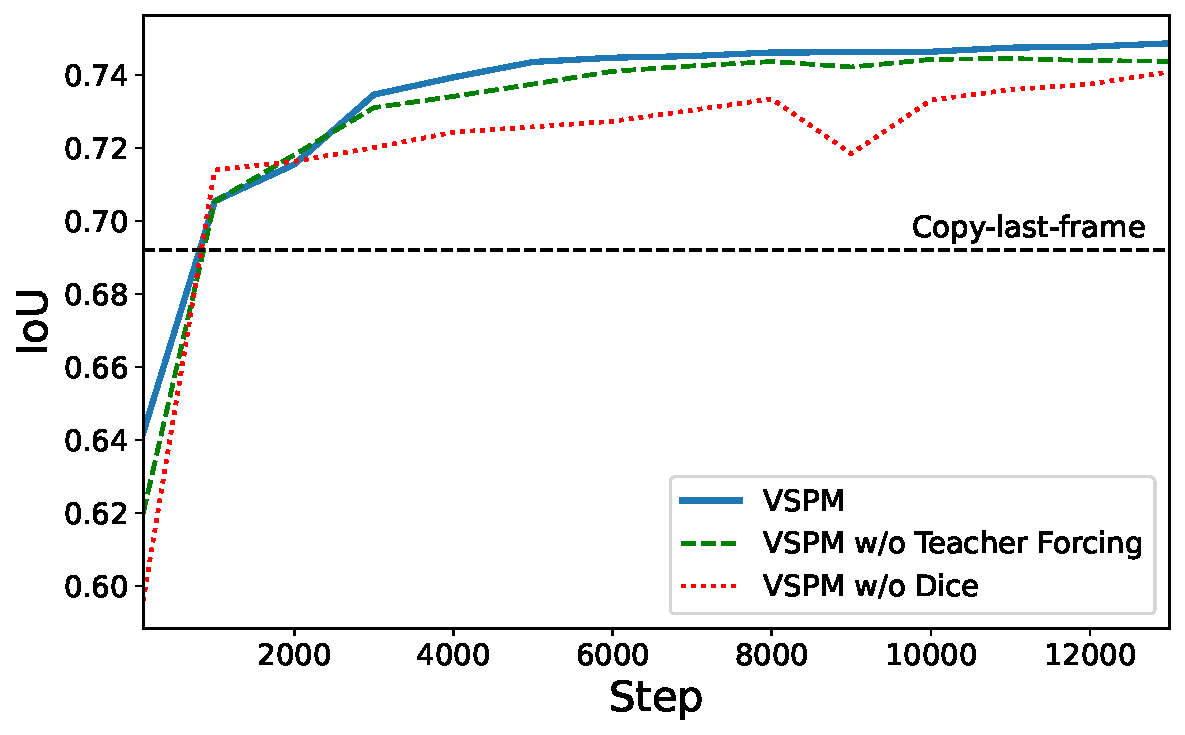
\includegraphics[width=0.95\linewidth]{pics/step-iou.pdf}
    \caption{
        \textbf{Ablation study on prediction IoU across horizons.} 
        Our full vehicle-specific prediction model~(VSPM) achieves consistently higher IoU compared to two ablated variants and a trivial copy-last-frame baseline. The x-axis represents the prediction horizon, and the y-axis represents the IoU score.
    }
    \label{fig:step_iou}
\end{figure}


\begin{figure*}[ht]
    \centering
    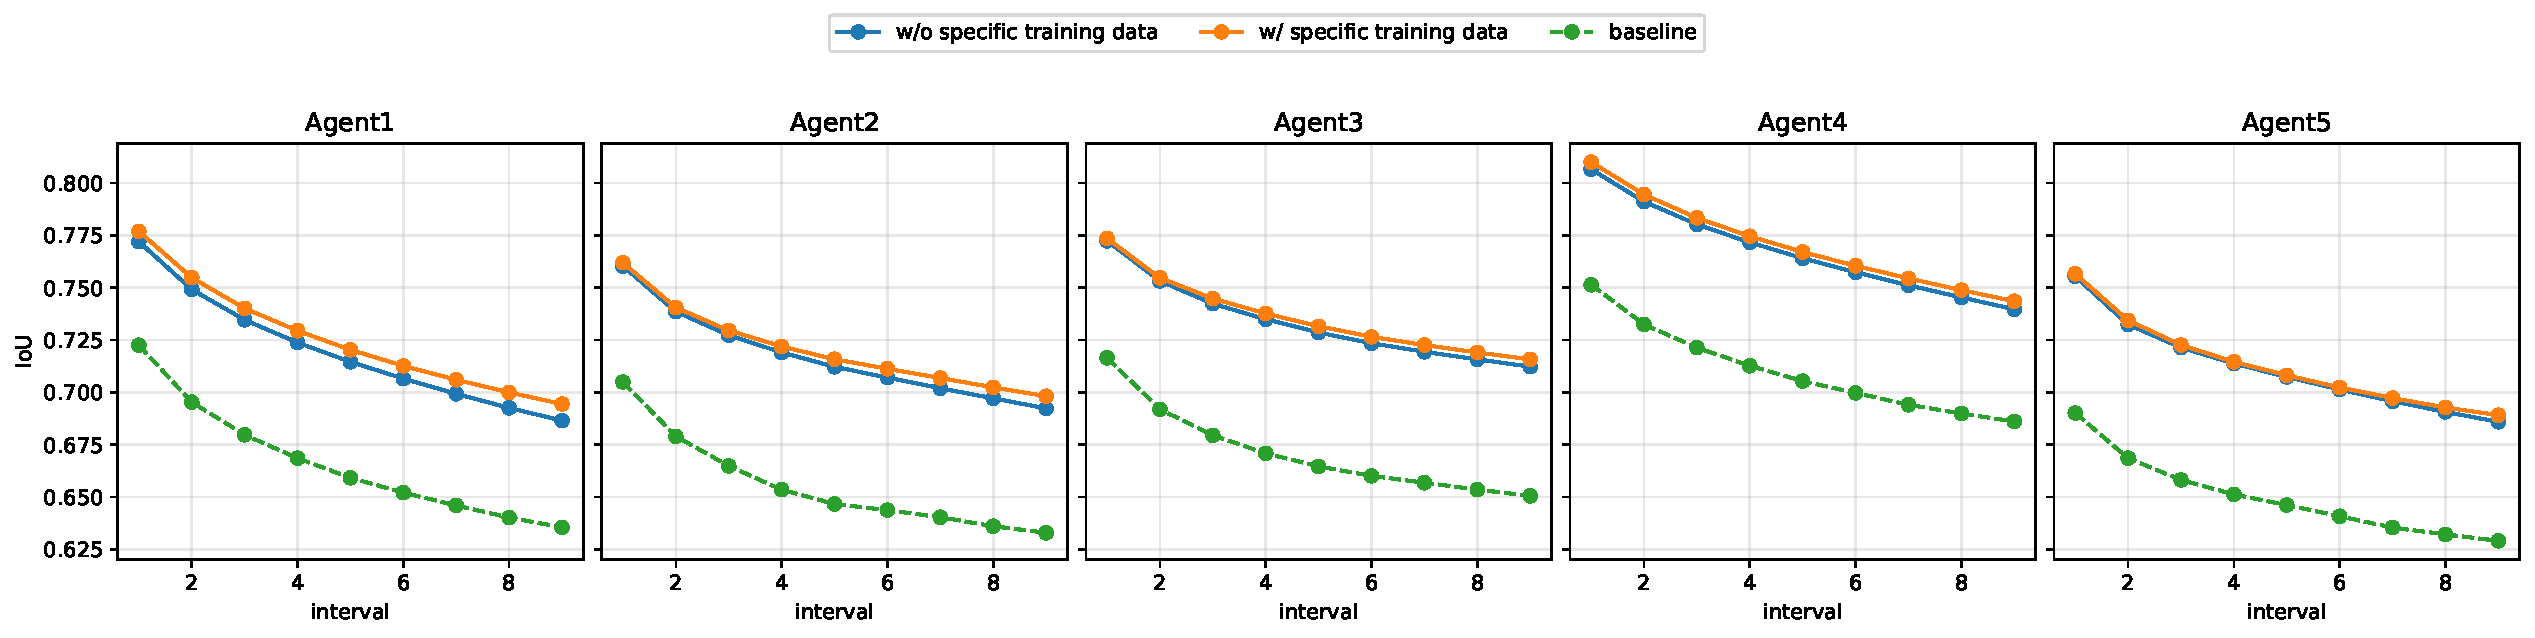
\includegraphics[width=0.95\linewidth]{pics/iou_vs_interval_5agents.pdf}
    \caption{
        \textbf{Comparison of prediction accuracy between generic and personalized models.} 
        IoU is reported under different latency intervals (measured in frames, with each frame representing 0.2 seconds) on the V2X-Sim dataset. Our personalization model consistently outperforms the generic model and the trivial copy-last-frame baseline. 
    }
    \label{fig:iou_interval}
\end{figure*}

\subsection{Experimental setup and evaluation metrics}
We conduct extensive experiments on both the V2X-Sim~\cite{li2022v2x} dataset and the real-world DAIR-V2X-C cooperative perception data to validate the effectiveness of the proposed dual-latency prediction compensation mechanism. Following prior works in cooperative perception, the V2X-Sim training and evaluation are performed on synchronized multi-vehicle data with simulated communication latency and computational latency. Our implementation is built upon the open-source V2VNet~\cite{wang2020v2vnet} and DiscoNet~\cite{li2021learning} framework, where we additionally integrate a lightweight prediction module at the transmitter side to compensate for both communication and computation latencies. For DAIR-V2X-C, we report official point-cloud detection baselines and additionally construct annotation-derived BEV occupancy sequences to evaluate the proposed VSPM and MST modules under real cooperative driving scenes.

For evaluation, we employ three categories of metrics. (1) To assess the accuracy of the vehicle-specific prediction models, we measure the Intersection-over-Union (IoU) between the predicted binary BEV occupancy grids and the ground-truth occupancy maps across different prediction horizons. We also report the IoU gain over the copy-last-frame baseline and the Dynamic IoU on changed BEV regions. (2) To quantify the system-level overhead, we record the reduction in both communication load and computational demand after introducing the proposed transmission scheme. (3) Finally, for the downstream perception fusion performance, we report Average Precision (AP) at IoU thresholds of 0.5 and 0.7, following standard practice in object detection benchmarks.
 



\subsection{Results analysis}
\subsubsection{\textbf{Vehicle-Specific Prediction Model}}
We first evaluate the effectiveness of the proposed prediction module in isolation, without involving any cooperative perception. Specifically, we compare the IoU between predicted and ground-truth occupancy maps under different prediction horizons, as shown in Fig.~\ref{fig:step_iou} and Fig.~\ref{fig:iou_interval}. In addition to conducting a detailed ablation study to quantify the impact of key design choices in our Visual Specific Prediction Module (VSPM), we compare the performance of our VSPM under two different configurations: one as a general model and the other as a specific model, which validates the importance of vehicle-specific in our framework.


\paragraph{Ablation Study}


Our full VSPM integrates scheduled teacher forcing, dynamic per-pixel weighting, and Dice regularization to improve prediction stability in both static and dynamic regions. It represents the main configuration of our model.

\textbf{VSPM w/o Teacher Forcing:}
To study the effect of teacher forcing, we disable scheduled sampling and instead always feed the model's own predictions as decoder inputs during training. This exposes the model to compounding prediction errors during rollout, providing a stress test of exposure bias.

\textbf{VSPM w/o Dice:}  
To examine the effect of addressing class imbalance, we remove the Dice loss while keeping all other components unchanged. Since occupancy prediction often suffers from the sparsity of dynamic objects, this ablation tests the necessity of Dice regularization for improving performance in foreground regions.

\textbf{Copy-last-frame Baseline:}  
We additionally include a trivial baseline that directly copies the previous observed occupancy map as the prediction for future horizons, without any learned dynamics modeling.

Figure~\ref{fig:step_iou} shows the IoU trajectories over prediction horizons. Our full VSPM consistently outperforms both ablations and the trivial baseline across all horizons. Notably, removing teacher forcing leads to a sharp IoU degradation in long-term predictions, while removing Dice yields a moderate performance drop in both near-term and far-horizon forecasts. These results validate the necessity of both components for accurate and stable occupancy prediction.



\paragraph{Effectiveness of VSPM}

Beyond the internal ablations, we further evaluate the overall impact of personalization by comparing three different prediction strategies:  
(1) a \textbf{generic model} trained solely on data from other vehicles without using any vehicle-specific information,  
(2) a \textbf{personalization model} trained on both generic multi-vehicle data and the receiver vehicle's historical data, and  
(3) a \textbf{copy-last-frame baseline} that simply reuses the most recent observation without any learned prediction.


 
As shown in Fig.~\ref{fig:iou_interval}, the personalization model achieves consistently higher IoU across all prediction horizons compared to the generic model and the copy-last-frame baseline. We highlight the following key findings:
\begin{itemize}[leftmargin=*,itemsep=0pt,parsep=0.2em,topsep=0.2em,partopsep=0.0em]
    \item Effectiveness of Personalization: Leveraging vehicle-specific historical data significantly improves prediction accuracy. At a $9$-frame latency, the personalization model consistently achieves higher IoU than the generic model across all scenarios.
    \item Limitations of Generic Models: Without access to the receiver vehicle's historical dynamics, the generic model struggles to adapt to diverse driving behaviors, leading to reduced performance as latency increases.
    \item Baseline Weakness: The copy-last-frame baseline suffers the most severe degradation, particularly for large latency, validating the necessity of learned temporal modeling.
\end{itemize}

These results confirm that VSPM offers a clear advantage over generic models under communication and computation latency constraints.


\begin{table*}[t]
\centering
\caption{Comparison of mAP@0.5 and mAP@0.7 under different \emph{communication and computation latency} settings on the V2X\textendash Sim dataset. Oracle and No Collaboration are reported only at the AVG columns (others are unavailable, shown as ``--''). Our method outperforms V2VNet across all latency conditions and surpasses the Oracle under zero latency.}
\begin{tabular}{c c *{14}{c}}
\toprule
\multirow{2}{*}{\textbf{Method}} & &
\multicolumn{7}{c}{\textbf{AP@0.5}} &
\multicolumn{7}{c}{\textbf{AP@0.7}} \\
\cmidrule(lr){3-9}\cmidrule(lr){10-16}
& \multicolumn{1}{c}{\diagbox{\small{Comp.}}{\small{Comm.}}} &
\textbf{AVG} & \textbf{0} & \textbf{1} & \textbf{2} & \textbf{3} & \textbf{4} & \textbf{5} &
\textbf{AVG} & \textbf{0} & \textbf{1} & \textbf{2} & \textbf{3} & \textbf{4} & \textbf{5} \\
\midrule
\textbf{Oracle} & -- &
\textit{64.91} & -- & -- & -- & -- & -- & -- &
\textit{57.26} & -- & -- & -- & -- & -- & -- \\
\textbf{No Collaboration} & -- &
49.90 & -- & -- & -- & -- & -- & -- &
44.21 & -- & -- & -- & -- & -- & -- \\
\midrule
\multirow{3}{*}{\textbf{V2VNet}} & 0 &
57.43 & 64.91 & 60.01 & 55.69 & 54.44 & 53.79 & 53.21 &
47.61 & 57.26 & 47.03 & 45.46 & 45.24 & 44.78 & 44.51 \\
& 2 &
54.63 & 55.45 & 54.91 & 54.73 & 54.55 & 54.23 & 53.89 &
45.20 & 45.29 & 45.40 & 45.35 & 45.27 & 45.05 & 44.82 \\
& 4 &
53.52 & 53.33 & 53.55 & 53.69 & 53.61 & 53.53 & 53.39 &
44.45 & 44.35 & 44.65 & 44.57 & 44.47 & 44.39 & 44.28 \\
\midrule
\multirow{3}{*}{\textbf{Ours}} & 0 &
64.41 & 67.45 & 65.16 & 64.06 & 63.56 & 63.19 & 63.04 &
56.41 & 58.64 & 57.12 & 56.25 & 55.68 & 55.43 & 55.34 \\
& 2 &
57.01 & 57.54 & 57.22 & 56.97 & 56.91 & 56.78 & 56.63 &
50.45 & 51.02 & 50.64 & 50.42 & 50.36 & 50.22 & 50.03 \\
& 4 &
56.07 & 56.40 & 56.21 & 56.15 & 55.96 & 55.90 & 55.80 &
49.45 & 49.87 & 49.65 & 49.46 & 49.39 & 49.25 & 49.09 \\
\bottomrule
\end{tabular}
\label{tab:map-upper-lower-v2v}
\end{table*}

\begin{figure*}[t]
    \centering
    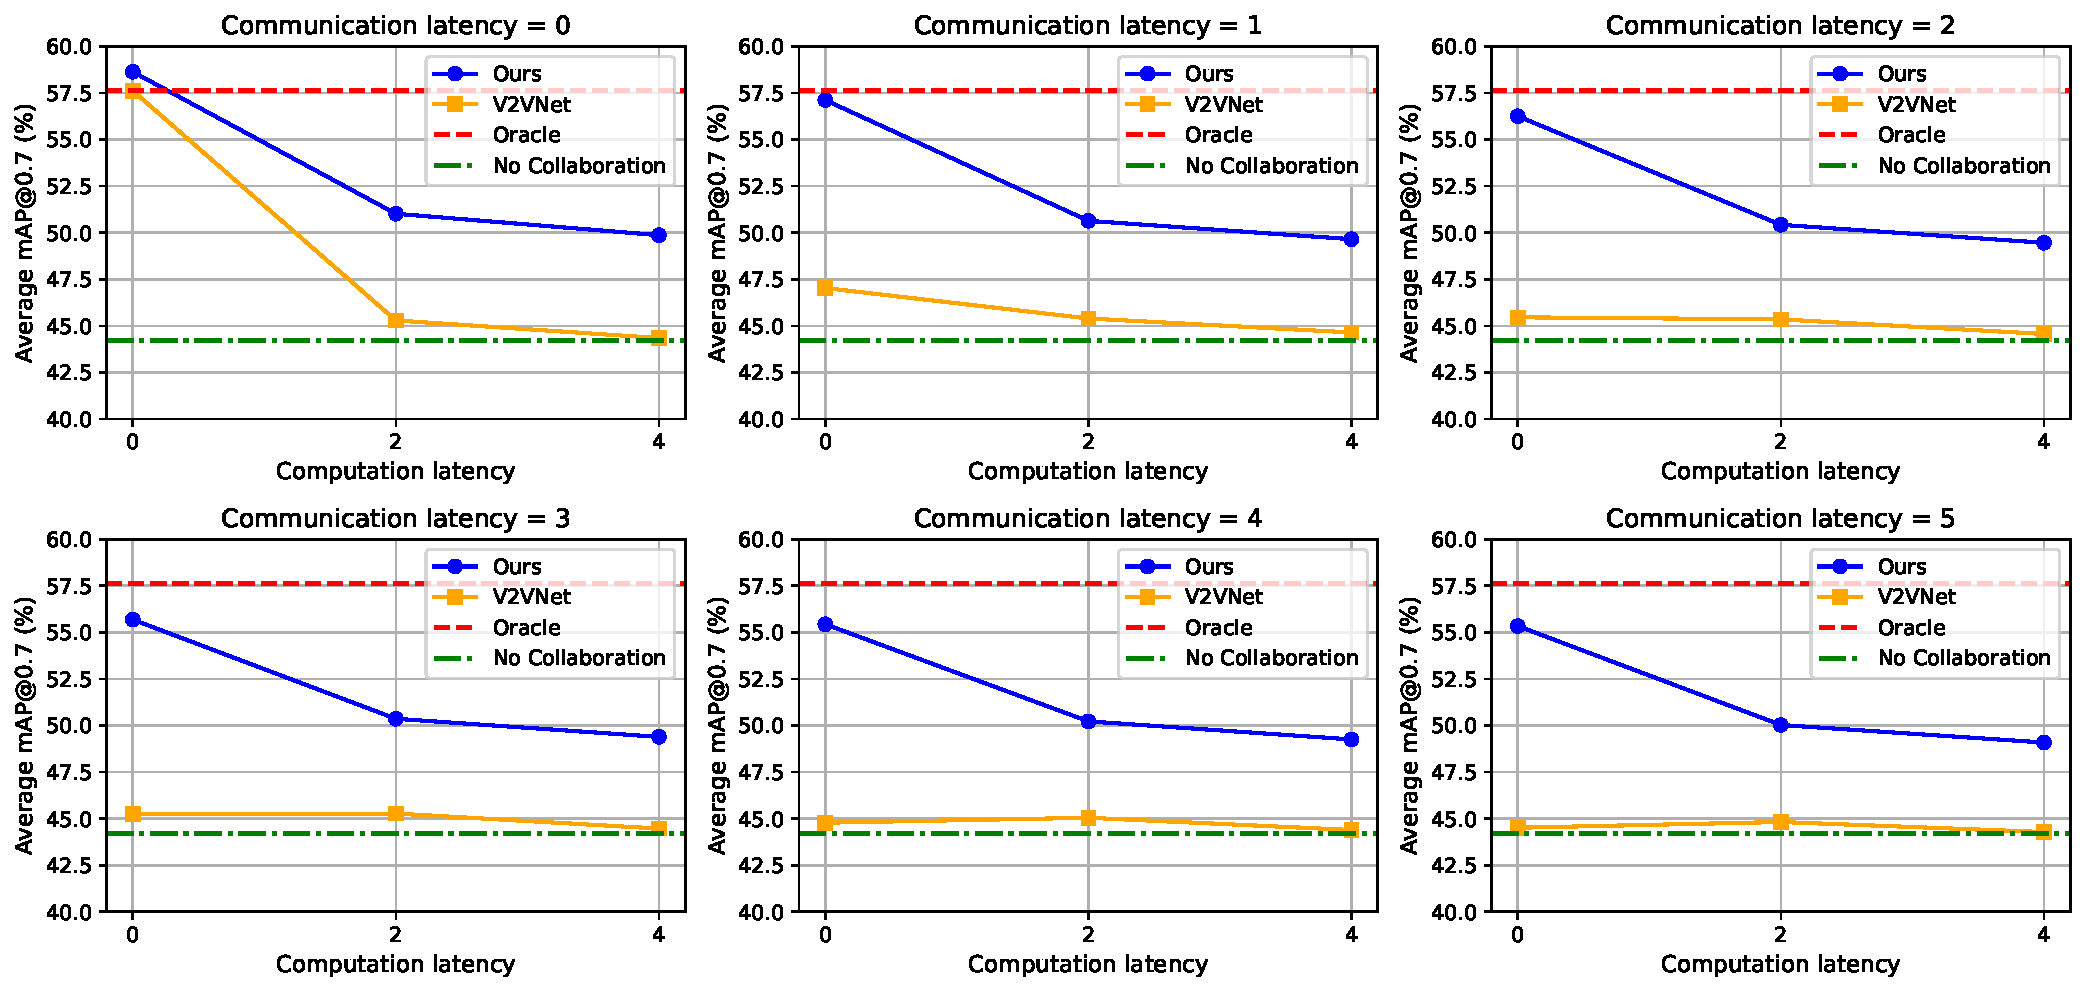
\includegraphics[width=0.95\linewidth]{pics/main_compare.pdf}
    \caption{Comparison of mAP@0.7 under varying communication and computation latency settings on the V2X-Sim dataset. Our method consistently outperforms the V2VNet baseline across all latency conditions and even surpasses the Oracle in the zero-latency scenario by leveraging richer historical information. Latency is measured in frames, with each frame representing 0.2 seconds.
    }
    \label{fig:0.7_lat}
\end{figure*}

\begin{figure*}[t]
    \centering
    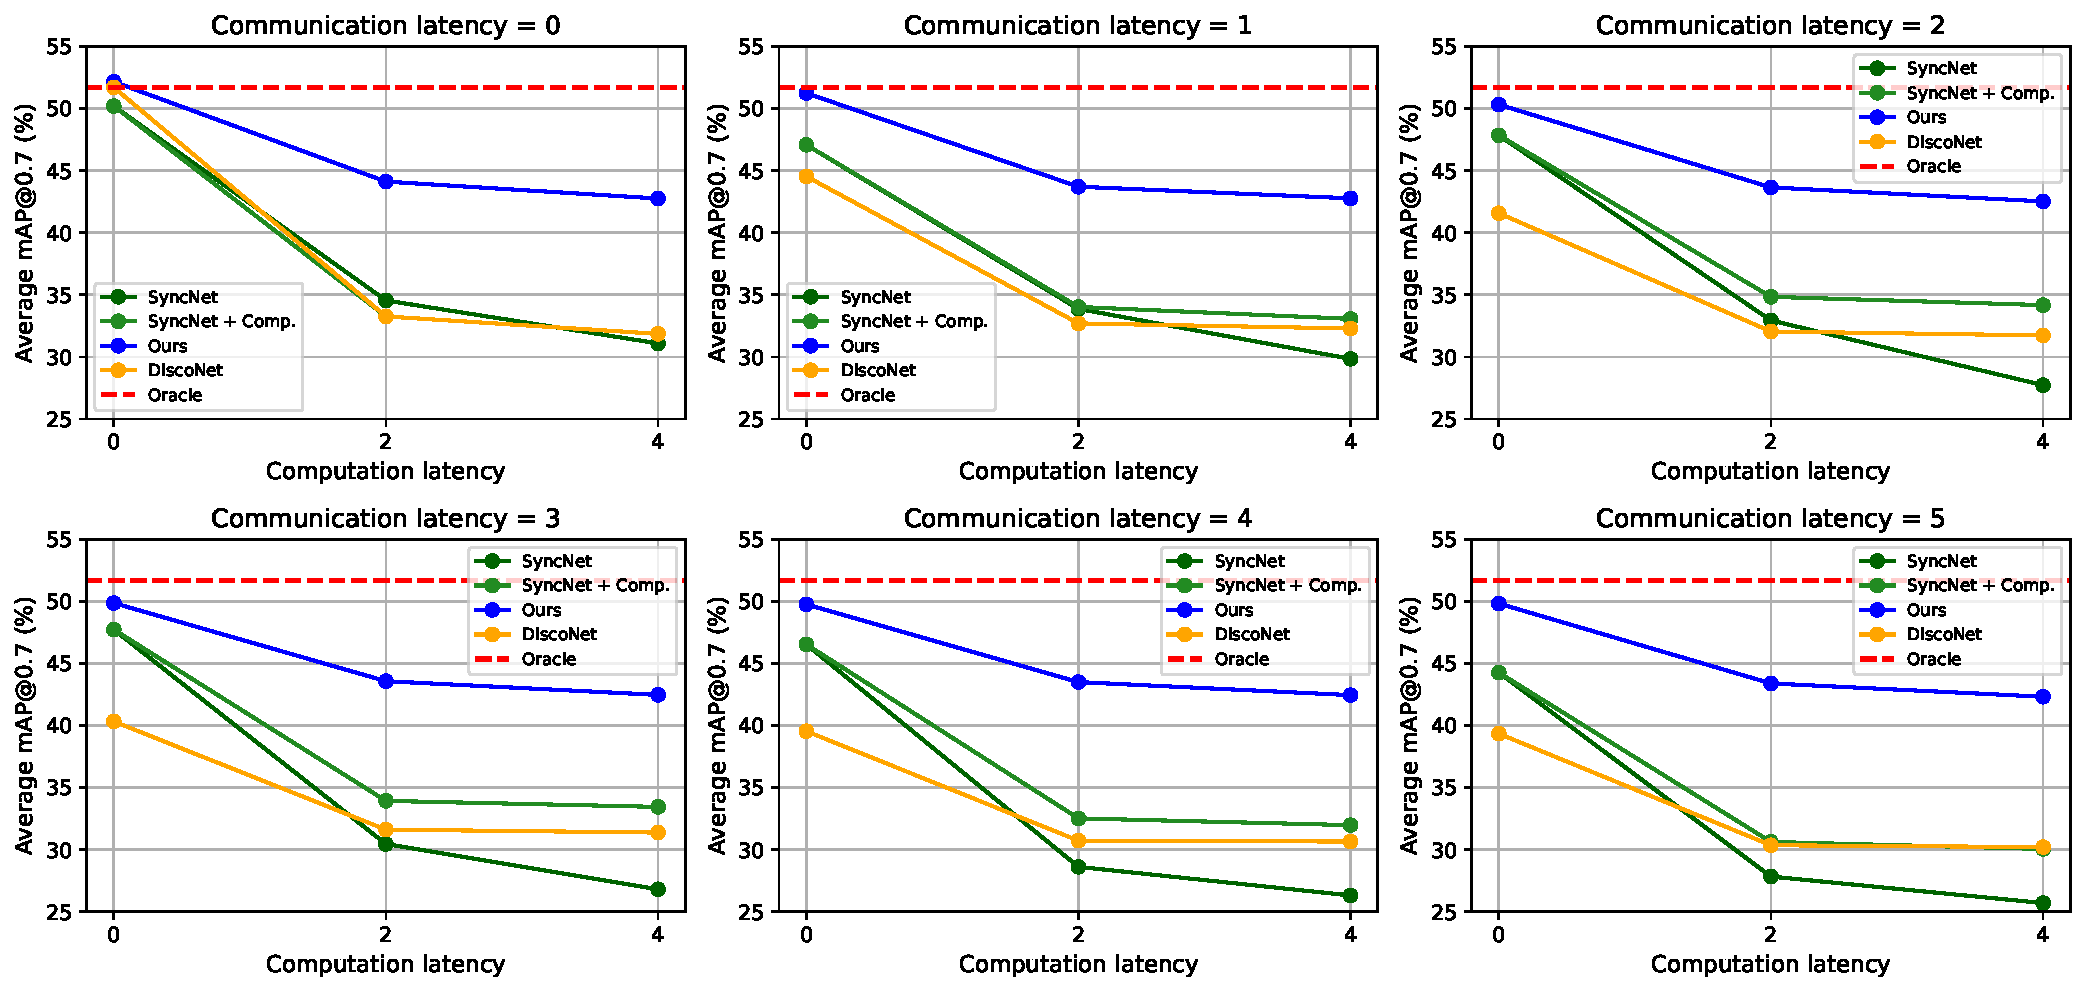
\includegraphics[width=0.95\linewidth]{pics/compare_disco-07}
    \caption{Comparison of mAP@0.7 under varying communication and computation latency settings on the V2X-Sim dataset. We compare four approaches: SyncNet, SyncNet + Comp., DiscoNet, Ours, and Oracle. Since the original SyncNet does not account for computation latency, we additionally present its extended results where computation latency is considered to provide a more comprehensive comparison. Latency is measured in frames, with each frame representing 0.2 seconds.
    }
    \label{fig:compare_syn}
\end{figure*}


\subsubsection{\textbf{Model State Transmission}}\\

We then investigate the efficiency gains brought by transmitting only compressed model states instead of feature-level data. Two aspects are considered: (i) the reduction of communication bandwidth consumption, and (ii) the alleviation of redundant computation at the receiver side. Both aspects are reported in tabular form to provide a clear quantitative comparison.
\paragraph{Changes in Communication Pressure}
\begin{table}[ht]
\centering
\caption{Comparison of Communication Pressure: Feature-Level Data vs. Compressed Model States}
\begin{tabular}{lcc}
\toprule
\textbf{Communication Data Type} & \textbf{Transmission Size} & \textbf{Reduction} \\
\midrule
Feature-Level Data & 1.9MB & - \\
Compressed Model States & 0.65MB & 65\% \\
\bottomrule
\end{tabular}

\label{tab:communication_pressure_comparison}
\end{table}

By compressing the model states and transmitting them instead of the feature-level data, we significantly alleviate the communication pressure. Specifically, in the Table~\ref{tab:communication_pressure_comparison}, the feature-level data (1.9MB) represents the data after fusing and processing perception information from multiple sensors of a transmitting vehicle. Using the int8pc compression method with temporal differencing, we reduced the size of the transmitted model states to 0.65MB (with an Normalized Mean Squared Error(NMSE) of 0.0054\%), resulting in a reduction of approximately 65\% in communication volume. This V2X-Sim comparison reports the original feature-level transmission setting, while the later DAIR-V2X-C MST table reports recurrent-state variants under a separate state-size profiling protocol. The two numbers therefore quantify different transmission formats rather than conflicting measurements. This transmission mechanism not only effectively reduces communication pressure but also provides the system with richer information, leading to more precise predictive compensation. 


\paragraph{Reducing Redundant Computation}
In this work, we propose a strategy where the encoder computation is offloaded to the transmitting vehicle, while the decoder computation is handled by the receiving vehicles. This distribution of computation has several key advantages in terms of reducing redundant computational load, particularly in a multi-agent system. 
When both the encoder and decoder computations are performed by each receiving vehicle, the redundancy increases with the number of receiving vehicles. Specifically, for each additional receiving vehicle, the encoder computation must be repeated, thereby leading to significant computational overhead. This redundancy becomes more pronounced as the number of receiving vehicles increases. In contrast, by offloading the encoder to the transmitting vehicle, only a single vehicle performs the encoder operation, while the receiving vehicles only execute the decoder. This leads to a significant reduction in computational redundancy.
In our method, the encoder computation is roughly 3 times more computationally expensive than the decoder computation (Table~\ref{tab:redundant_computation_comparison}). So, if we have a system with 5 vehicles, and 4 of them are receiving vehicles, the redundancy caused by the repeated execution of the encoder operation across these receiving vehicles results in a total computational overhead equivalent to three times the encoder's calculation. This redundancy represents about 57.1\% of the total computational load in the system. Therefore, by offloading the encoder to the transmitting vehicle and allowing only the decoder to run on the receiving vehicles, we achieve a significant reduction in computational redundancy, optimizing overall system efficiency.

%encoder：1600000flops decoder：50000flops Redundant encoder computation=3×1,600,000=4,800,000FLOPs  Total computation for 4 receiving vehicles=4×2,100,000=8,400,000FLOPs  48/84=57.1%
\begin{table}[ht]
\centering
\caption{Comparison of Redundant Computation in the System}
\begin{tabular}{lcc}
\toprule
\textbf{Computation Type} & \textbf{Computation (MFLOPs)} \\
\midrule
Encoder (per vehicle) & 1.6 \\
Decoder (per vehicle) & 0.5 \\
Redundant Encoder (for 3 vehicles) & 4.8 \\
Total (for 4 receiving vehicles) & 8.4 \\
\midrule
Redundant Percentage & 57.1\% \\
\bottomrule
\end{tabular}
\label{tab:redundant_computation_comparison}
\end{table}

%FLOPs stands for Floating Point Operations, which is a measure of computational performance. It refers to the number of mathematical operations (such as additions, multiplications, etc.) involving floating-point numbers that are performed by a processor or algorithm.

\subsubsection{\textbf{Dual-latency Perceptive Compensation Fusion}}
Finally, we evaluate the end-to-end performance of cooperative perception under dual-latency settings, i.e., simultaneous communication and computation latencies. To better approximate real-world deployment, we vary the latency configurations to emulate different compression ratios. Our method is compared against four baselines: SyncNet~\cite{lei2022latency}, an oracle (ideal V2VNet~\cite{wang2020v2vnet} or DiscoNet~\cite{li2021learning} without latency), a lower-bound (V2VNet~\cite{wang2020v2vnet} or DiscoNet~\cite{li2021learning} with latency but without compensation), and the single-agent V2VNet~\cite{wang2020v2vnet} or DiscoNet~\cite{li2021learning} without cooperation. Results are reported in terms of AP@0.5/0.7 across all latency settings. Both tabular and graphical comparisons demonstrate that the proposed transmitter-side compensation achieves consistently superior performance in diverse latency scenarios.

\begin{table*}[t]
\centering
\caption{Comparison of mAP@0.5 and mAP@0.7 under different \emph{communication and computation latency} settings on the V2X\textendash Sim dataset. Oracle is reported only at the AVG columns (others are unavailable, shown as ``--'').}
\begin{tabular}{c c *{14}{c}}
\toprule
\multirow{2}{*}{\textbf{Method}} & &
\multicolumn{7}{c}{\textbf{AP@0.5}} &
\multicolumn{7}{c}{\textbf{AP@0.7}} \\
\cmidrule(lr){3-9}\cmidrule(lr){10-16}
& \multicolumn{1}{c}{\diagbox{\small{Comp.}}{\small{Comm.}}} &
\textbf{AVG} & \textbf{0} & \textbf{1} & \textbf{2} & \textbf{3} & \textbf{4} & \textbf{5} &
\textbf{AVG} & \textbf{0} & \textbf{1} & \textbf{2} & \textbf{3} & \textbf{4} & \textbf{5} \\
\midrule
\textbf{Oracle} & -- &
\textit{56.62} & -- & -- & -- & -- & -- & -- &
\textit{51.70} & -- & -- & -- & -- & -- & -- \\
\midrule
\multirow{3}{*}{\textbf{SyncNet}} & 0 &
55.07 & 56.62 & 53.49 & 55.73 & 55.72 & 54.90 & 52.56 &
47.27 & 50.20 & 47.08 & 47.84 & 47.72 & 46.53 & 44.26 \\
& 2 &
38.34 & 41.14 & 40.98 & 40.04 & 37.87 & 35.60 & 34.41 &
31.38 & 34.55 & 33.87 & 32.94 & 30.45 & 28.62 & 27.83 \\
& 4 &
34.62 & 37.91 & 36.46 & 34.72 & 33.89 & 32.83 & 31.90 &
27.91 & 31.09 & 29.84 & 27.73 & 26.81 & 26.31 & 25.70 \\
\midrule
\multirow{3}{*}{\textbf{SyncNet w/ Comp.}} & 0 &
55.07 & 56.62 & 53.49 & 55.73 & 55.72 & 54.90 & 52.56 &
47.27 & 50.20 & 47.08 & 47.84 & 47.72 & 46.53 & 44.26 \\
& 2 &
39.94 & 41.25 & 39.73 & 41.52 & 40.53 & 39.28 & 37.35 &
33.20 & 33.26 & 34.02 & 34.84 & 33.93 & 32.52 & 30.62 \\
& 4 &
38.55 & 38.65 & 38.25 & 40.34 & 39.53 & 38.21 & 36.31 &
32.43 & 31.86 & 33.06 & 34.17 & 33.44 & 31.97 & 30.06 \\
\midrule
\multirow{3}{*}{\textbf{DiscoNet}} & 0 &
51.46 & 56.62 & 54.88 & 51.24 & 49.46 & 48.60 & 47.94 &
42.84 & 51.70 & 44.53 & 41.57 & 40.32 & 39.54 & 39.34 \\
& 2 &
39.19 & 41.25 & 41.03 & 39.75 & 38.91 & 37.38 & 36.80 &
31.78 & 33.26 & 32.70 & 32.05 & 31.61 & 30.72 & 30.36 \\
& 4 &
37.87 & 38.65 & 39.41 & 38.35 & 37.70 & 36.85 & 36.25 &
31.35 & 31.86 & 32.29 & 31.73 & 31.38 & 30.65 & 30.21 \\
\midrule
\multirow{3}{*}{\textbf{Ours}} & 0 &
54.52 & 56.83 & 55.09 & 54.11 & 53.83 & 53.56 & 53.70 &
50.52 & 52.16 & 51.24 & 50.32 & 49.86 & 49.75 & 49.82 \\
& 2 &
48.15 & 48.59 & 48.22 & 48.16 & 48.11 & 47.92 & 47.89 &
43.65 & 44.11 & 43.70 & 43.65 & 43.57 & 43.49 & 43.39 \\
& 4 &
46.99 & 47.31 & 47.13 & 46.95 & 46.98 & 46.85 & 46.75 &
42.54 & 42.75 & 42.77 & 42.52 & 42.46 & 42.44 & 42.31 \\
\bottomrule
\end{tabular}
\label{tab:map-upper-lower-disco}
\end{table*}

%In Table~\ref{tab:map-upper-lower}, we present a comprehensive performance comparison between our method based on V2VNet~\cite{wang2020v2vnet} and various baselines under different \emph{communication} and \emph{computation} latency settings. The reported mAP@0.5 and mAP@0.7 are averaged over all test cases, considering Communication latency = 0--5 and Computation latency = 0--4. Overall, our method consistently achieves superior performance across all latency conditions. Specifically, compared to the V2VNet baseline, our approach improves the averaged mAP@0.5 by approximately \textbf{3\%--7\%} and the averaged mAP@0.7 by approximately \textbf{5\%--10\%}, demonstrating its robustness under various latency scenarios.

In Table~\ref{tab:map-upper-lower-v2v}, we present a comprehensive performance comparison between our method based on V2VNet~\cite{wang2020v2vnet} and various baselines under different \emph{communication} and \emph{computation} latency settings. The reported mAP@0.5 and mAP@0.7 are averaged over all test cases, considering Communication latency = 0--5 and Computation latency = 0--4.

From the V2VNet~\cite{wang2020v2vnet} results, it can be seen that as the computation latency increases, the performance of V2VNet without the dual-latency prediction compensation mechanism declines significantly. Even with just a 2-frame computation latency, there is a considerable performance fluctuation, with a nearly \textbf{12\%} drop in AP@0.7. Under computation latency = 4 and communication latency = 5, the AP@0.7 results of V2VNet without compensation are already very close to the results of no collaboration. These findings highlight that in cooperative perception scenarios, both communication latency and computation latency are crucial issues that cannot be overlooked, effectively demonstrating the significance of our dual-latency prediction compensation mechanism.

Meanwhile, our method consistently achieves superior performance across all latency conditions. Specifically, compared to the V2VNet baseline, our approach improves the averaged mAP@0.5 by approximately \textbf{3\%--7\%} and the averaged mAP@0.7 by approximately \textbf{5\%--9\%}, demonstrating its robustness under various latency scenarios. Even in adverse conditions with a communication latency of 5, our dual-latency compensation mechanism improves the V2VNet baseline by about \textbf{10\%}, falling short of the ideal scenario by \textbf{less than 2\%}. Additionally, when the computation latency is significantly large at 4, our framework achieves a 5.52\% improvement in AP@0.7, effectively proving that our dual-latency prediction compensation mechanism greatly enhances the robustness of V2VNet under dual latency conditions.


Furthermore, as illustrated in Figure~\ref{fig:0.7_lat}, which vividly showcases the data from Table~\ref{tab:map-upper-lower-v2v}, our method even \emph{surpasses the Oracle performance} in the ideal zero-latency scenario. This notable gain can be attributed to leveraging \emph{richer historical information}, which provides additional context for collaborative perception and mitigates temporal inconsistency. Importantly, under \emph{all} latency settings, our method maintains a consistent performance advantage over the V2VNet baseline, confirming its effectiveness in handling delayed information. Moreover, we can observe that when the communication latency is greater than 1 and the computation latency is present, the results of the V2VNet baseline are very close to those of no collaboration, which diminishes the benefits of inter-agent communication. The results once again emphasize the significant impact of dual latency on the accuracy of cooperative perception.

%It is also worth noting that when computation latency is ignored, the performance of V2VNet approaches the lower bound established by the No Collaboration setting. This observation highlights the \emph{critical importance of accounting for computation latency} when designing collaborative perception systems, as neglecting it can significantly diminish the benefits of inter-agent communication.
%In Figure~\ref{fig:compare_syn}, we compare our compensation mechanism with SyncNet~\cite{lei2022latency} on DiscoNet~\cite{li2021learning} under different communication and computation latency settings. The original SyncNet does not account for computation latency in its design. To provide a fair and comprehensive comparison, we evaluate two variants of SyncNet: one that strictly follows the original implementation and another extended version, SyncNet+Comp, where computation latency is explicitly considered. The results demonstrate that our method consistently outperforms both SyncNet variants under nearly all latency conditions. Moreover, SyncNet+Comp achieves superior performance compared to the original SyncNet in the vast majority of scenarios, underscoring the significance of properly modeling computation latency for collaborative perception.
In Table~\ref{tab:map-upper-lower-disco}, we further present the results based on DiscoNet~\cite{li2021learning} and compare them against multiple baselines. Consistent with the findings on V2VNet~\cite{wang2020v2vnet}, the performance of the original DiscoNet degrades significantly as the computation and communication latencies increase, highlighting that the impact of both communication and computation latency on system performance is not an isolated phenomenon in cooperative perception.

In contrast, our method consistently demonstrates stable advantages across all latency configurations. On average, our approach improves the baseline DiscoNet by approximately \textbf{3\%--9\%} in mAP@0.5 and \textbf{8\%--12\%} in mAP@0.7, further validating the effectiveness of the proposed dual-latency prediction compensation mechanism in enhancing robustness. Even under the extreme condition of communication latency = 5 and computation latency = 4, our method maintains a clear margin over the baseline, underscoring its resilience in challenging latency environments.

To further evaluate the effectiveness of our framework, we also compare it with SyncNet~\cite{lei2022latency} and its extended variant SyncNet+Comp. As shown in Table~\ref{tab:map-upper-lower-disco}, the original SyncNet does not account for computation latency in its design, and thus its performance drops rapidly as latency grows. In contrast, SyncNet+Comp achieves noticeable improvements over the original SyncNet in most scenarios, verifying the importance of explicitly modeling computation latency. Nevertheless, our method consistently outperforms both SyncNet variants under all latency conditions, further demonstrating the generality and superiority of the proposed compensation mechanism.

In Figure~\ref{fig:compare_syn}, we illustrate the trends of mAP@0.7 under different communication latencies as computation latency increases. The results clearly indicate that the performance of SyncNet degrades sharply under high-latency conditions, whereas our framework consistently sustains a higher level of accuracy. This observation not only confirms the adaptability of the proposed dual-latency prediction compensation mechanism to DiscoNet but also reinforces the critical importance of dual-latency modeling for collaborative perception.

In summary, whether built upon V2VNet~\cite{wang2020v2vnet} or DiscoNet~\cite{li2021learning}, our method consistently demonstrates significant and robust advantages under dual-latency settings. Compared to existing approaches, the proposed compensation mechanism effectively mitigates performance degradation across diverse latency configurations while maintaining high perception accuracy. More importantly, even under complex and adverse latency conditions, our framework continues to deliver stable improvements over baseline methods, fully validating its practicality and robustness for real-world deployment.

\subsubsection{\textbf{DAIR-V2X-C Real-World Validation}}
To further examine whether the proposed mechanism remains valid beyond the simulated V2X-Sim setting, we conduct additional experiments on DAIR-V2X-C. This part contains two complementary evaluations. First, we run official cooperative detection baselines to quantify how real DAIR point-cloud detection performance changes with communication delay. Second, we evaluate our VSPM and MST components on DAIR annotation-derived BEV occupancy sequences, which allows the same latency-compensation logic and prediction metrics to be tested on real cooperative scenes. These two DAIR evaluations use different metrics and should be interpreted separately: the official baselines report detection AP, while our DAIR VSPM/MST evaluation reports BEV forecasting IoU and does not claim end-to-end detection AP for our method.

\begin{table*}[t]
\centering
\scriptsize
\caption{Representative DAIR-V2X-C official detection baselines. Delay is measured in frames.}
\label{tab:dair-official-baselines}
\begin{tabular}{lrrrrrr}
\toprule
Method & $k$ & 3D@0.5 & 3D@0.7 & BEV@0.5 & BEV@0.7 & Comm. B \\
\midrule
Vehicle only & 0 & 48.03 & 35.08 & 52.24 & 46.51 & 0.00 \\
Infrastructure only & 0 & 17.60 & 7.06 & 27.34 & 14.42 & 478.56 \\
Late fusion + TCLF & 0 & 55.98 & 40.01 & 62.00 & 54.11 & 911.96 \\
Late fusion + TCLF & 3 & 52.14 & 36.57 & 57.80 & 49.46 & 885.55 \\
Late fusion + TCLF & 5 & 51.29 & 36.30 & 56.75 & 48.71 & 861.65 \\
Late fusion w/o comp. & 1 & 53.73 & 36.88 & 59.90 & 50.11 & 478.76 \\
Late fusion w/o comp. & 3 & 51.36 & 36.25 & 56.90 & 48.80 & 477.40 \\
Late fusion w/o comp. & 5 & 50.87 & 36.17 & 56.18 & 48.36 & 466.53 \\
Early fusion & 0 & 62.61 & 37.50 & 68.94 & 59.02 & 2284.16 \\
Early fusion & 2 & 54.62 & 32.17 & 61.07 & 50.04 & 2316.11 \\
Early fusion & 5 & 50.93 & 30.98 & 56.47 & 46.99 & 2496.60 \\
\bottomrule
\end{tabular}
\end{table*}


\begin{figure}[t]
    \centering
    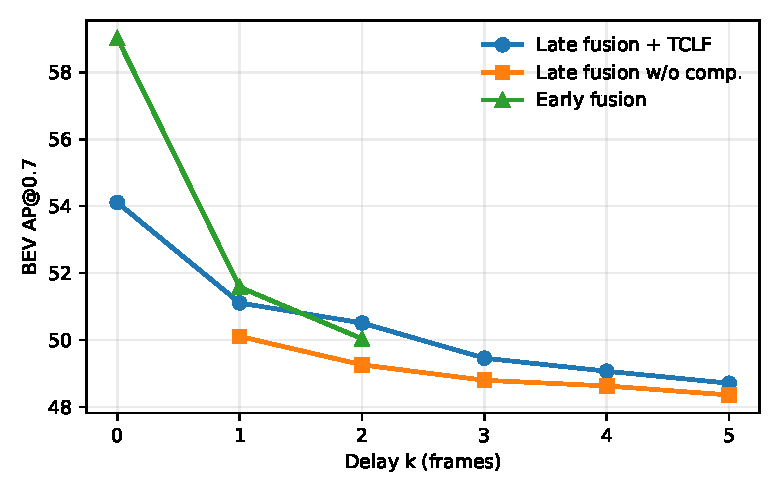
\includegraphics[width=0.95\linewidth]{pics/dair_official_delay.pdf}
    \caption{BEV AP@0.7 of DAIR-V2X-C official detection baselines under different delay settings. The results show that real cooperative detection accuracy degrades as stale information is used, while time-compensated late fusion remains more stable than uncompensated late fusion at larger delays.}
    \label{fig:dair-official-delay}
\end{figure}

Table~\ref{tab:dair-official-baselines} and Fig.~\ref{fig:dair-official-delay} summarize representative DAIR-V2X-C official detection results. Compared with vehicle-only perception, cooperative fusion improves both 3D and BEV AP, confirming the value of V2X information in real scenes. At the same time, the degradation from $k=0$ to larger delay values shows that delayed cooperative messages do hurt detection accuracy. The time-compensated late-fusion (TCLF) baseline maintains higher BEV AP@0.7 than the uncompensated late-fusion baseline at larger delays, which supports the central motivation of explicitly modeling latency in real cooperative perception. Early fusion is used here as a high-communication official reference rather than as a strict upper bound, since its performance also degrades under large delay.

\begin{table*}[t]
\centering
\scriptsize
\caption{DAIR-V2X label-derived BEV delay and system ablation.}
\label{tab:dair-delay-system}
\begin{tabular}{llrrrrr}
\toprule
Setting & Mode & Cases & IoU & Copy & $\Delta$IoU & Dyn. IoU \\
\midrule
T10\_n10 ckpt 15000 & no\_comp & 30 & 0.1945 & 0.1945 & 0.0000 & 0.0497 \\
T10\_n10 ckpt 15000 & comm\_only & 30 & 0.2960 & 0.1945 & 0.1015 & 0.2380 \\
T10\_n10 ckpt 15000 & comp\_only & 30 & 0.2784 & 0.1945 & 0.0839 & 0.2053 \\
T10\_n10 ckpt 15000 & dual & 30 & 0.4097 & 0.1945 & 0.2153 & 0.4436 \\
T10\_n10 ckpt 15000 & oracle & 30 & 1.0000 & 0.1945 & 0.8055 & 1.0000 \\
T10\_n5 ckpt 16000 & no\_comp & 15 & 0.2857 & 0.2857 & 0.0000 & 0.0836 \\
T10\_n5 ckpt 16000 & comm\_only & 15 & 0.3956 & 0.2857 & 0.1099 & 0.2672 \\
T10\_n5 ckpt 16000 & comp\_only & 15 & 0.3956 & 0.2857 & 0.1099 & 0.2672 \\
T10\_n5 ckpt 16000 & dual & 15 & 0.5207 & 0.2857 & 0.2350 & 0.4830 \\
T10\_n5 ckpt 16000 & oracle & 15 & 1.0000 & 0.2857 & 0.7143 & 1.0000 \\
\bottomrule
\end{tabular}
\end{table*}


\begin{figure}[t]
    \centering
    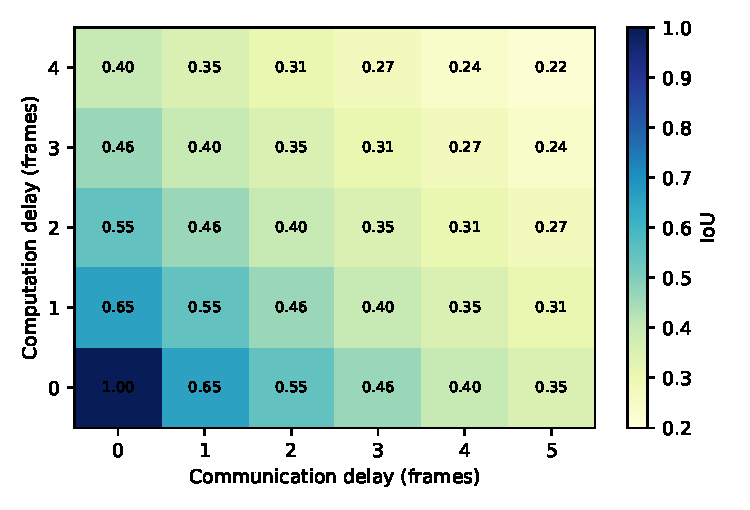
\includegraphics[width=0.95\linewidth]{pics/dair_delay_heatmap.pdf}
    \caption{DAIR-V2X-C label-derived BEV IoU of the proposed dual-latency compensation under the full $T10\_n10$ latency grid. The x-axis is communication delay and the y-axis is computation delay, both measured in frames.}
    \label{fig:dair-delay-heatmap}
\end{figure}

Table~\ref{tab:dair-delay-system} reports the system-level DAIR delay ablation. For the full $T10\_n10$ setting, the dual-latency mode achieves an average IoU of 0.4097, compared with 0.1945 for no compensation, 0.2960 for communication-only compensation, and 0.2784 for computation-only compensation. This full-grid setting is the main evidence for separating communication-only, computation-only, and joint compensation. For the shorter $T10\_n5$ setting, the supported latency subset is symmetric for the single-delay modes, so we use it primarily as a short-horizon confirmation: the dual-latency mode reaches 0.5207 IoU and improves over the no-compensation setting by 0.2350 IoU. These results demonstrate that communication and computation delays should be compensated jointly rather than treated as isolated effects. Fig.~\ref{fig:dair-delay-heatmap} further shows the expected trend that prediction difficulty increases as the total target horizon becomes larger.

\begin{table}[t]
\centering
\scriptsize
\caption{MST communication-state trade-off on DAIR-V2X label-derived BEV.}
\label{tab:dair-mst-tradeoff}
\begin{tabular}{lrrrrrr}
\toprule
Variant & MiB/agent & Reduction & ms & IoU & $\Delta$IoU & Dyn. IoU \\
\midrule
ConvLSTM state & 16.000 & 1.0$\times$ & 3.59 & 0.5188 & 0.2469 & 0.4646 \\
GRU FP16 & 4.000 & 4.0$\times$ & 4.40 & 0.5551 & 0.2833 & 0.5240 \\
DS64 FP16 & 0.250 & 64.0$\times$ & 4.21 & 0.6066 & 0.3348 & 0.5888 \\
Bottleneck12 & 0.250 & 64.0$\times$ & 4.31 & 0.6021 & 0.3302 & 0.5682 \\
\bottomrule
\end{tabular}
\end{table}


\begin{figure}[t]
    \centering
    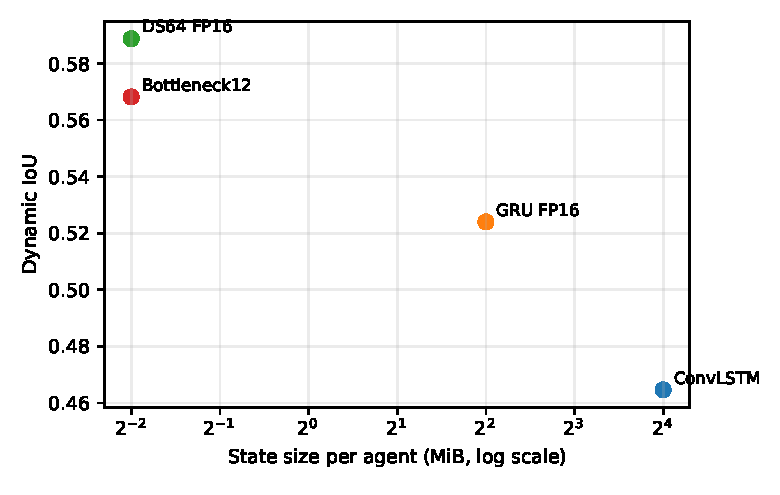
\includegraphics[width=0.95\linewidth]{pics/dair_mst_pareto.pdf}
    \caption{Bandwidth-performance trade-off of MST variants on DAIR-V2X-C label-derived BEV. Smaller state size reduces communication and cache pressure; Dynamic IoU reports prediction quality on changed BEV regions.}
    \label{fig:dair-mst-pareto}
\end{figure}

Table~\ref{tab:dair-mst-tradeoff} and Fig.~\ref{fig:dair-mst-pareto} analyze whether MST reduces communication-state cost without invalidating prediction quality. The original ConvLSTM hidden and cell states require 16.0 MiB per agent. The DS64-FP16 and Bottleneck12 variants reduce the recurrent state to 0.25 MiB per agent, corresponding to a $64\times$ reduction, while achieving higher IoU and Dynamic IoU than the uncompressed ConvLSTM-state baseline. This 0.25 MiB/agent value is the profiled DAIR recurrent-state footprint, whereas Table~\ref{tab:communication_pressure_comparison} reports a separate V2X-Sim feature-level transmission comparison. This indicates that the transmitted state can be compact while still preserving the temporal information needed for compensation.

\begin{table}[t]
\centering
\scriptsize
\caption{History length and rollout-horizon sensitivity on DAIR-V2X label-derived BEV.}
\label{tab:dair-sensitivity}
\begin{tabular}{lrrrr}
\toprule
Setting & Best step & IoU & $\Delta$IoU & Dyn. IoU \\
\midrule
T5\_n5 & 16650 & 0.5183 & 0.2464 & 0.4427 \\
our\_method\_T10\_n5 & 16140 & 0.5164 & 0.2446 & 0.4465 \\
T20\_n5 & 28000 & 0.5237 & 0.2522 & 0.4564 \\
T30\_n5 & 52000 & 0.5230 & 0.2519 & 0.4741 \\
T10\_n3 & 16350 & 0.5954 & 0.2229 & 0.4318 \\
our\_method\_T10\_n10 & 15630 & 0.3853 & 0.2105 & 0.3834 \\
T10\_n15 & 29000 & 0.3065 & 0.1722 & 0.3385 \\
\bottomrule
\end{tabular}
\end{table}


Table~\ref{tab:dair-sensitivity} studies the sensitivity to history length $T$ and prediction rollout horizon $n$. With $n=5$, increasing $T$ from 5 to 20 or 30 provides only moderate changes, which suggests that the default history length is not a fragile choice. In contrast, increasing the rollout horizon from $n=3$ to $n=10$ or $n=15$ clearly lowers absolute IoU, because long-horizon BEV forecasting is harder and covers larger communication/computation delay. This trend is consistent with the latency heatmap and explains why the short-horizon model is used for high-accuracy compensation while the $T10\_n10$ model is used to cover the full delay grid.

\begin{table*}[t]
\centering
\scriptsize
\caption{Robustness of DAIR-V2X VSPM under packet loss and BEV perturbations.}
\label{tab:dair-robustness}
\begin{tabular}{llrrrr}
\toprule
Setting & Condition & IoU & Copy & $\Delta$IoU & Dyn. IoU \\
\midrule
T10\_n5 ckpt 16000 & clean & 0.5478 & 0.2771 & 0.2707 & 0.4733 \\
T10\_n5 ckpt 16000 & packet\_loss\_0.3 & 0.4411 & 0.2443 & 0.1968 & 0.3490 \\
T10\_n5 ckpt 16000 & packet\_loss\_0.5 & 0.3476 & 0.2126 & 0.1351 & 0.2497 \\
T10\_n5 ckpt 16000 & dropout\_0.2 & 0.4867 & 0.2368 & 0.2500 & 0.4436 \\
T10\_n5 ckpt 16000 & false\_positive\_0.005 & 0.5082 & 0.2140 & 0.2942 & 0.4268 \\
T10\_n10 ckpt 15000 & clean & 0.4057 & 0.1709 & 0.2348 & 0.4291 \\
T10\_n10 ckpt 15000 & packet\_loss\_0.3 & 0.3261 & 0.1540 & 0.1721 & 0.3267 \\
T10\_n10 ckpt 15000 & packet\_loss\_0.5 & 0.2569 & 0.1366 & 0.1203 & 0.2413 \\
T10\_n10 ckpt 15000 & dropout\_0.2 & 0.3742 & 0.1471 & 0.2271 & 0.4050 \\
T10\_n10 ckpt 15000 & false\_positive\_0.005 & 0.3833 & 0.1357 & 0.2476 & 0.3755 \\
\bottomrule
\end{tabular}
\end{table*}


\begin{figure}[t]
    \centering
    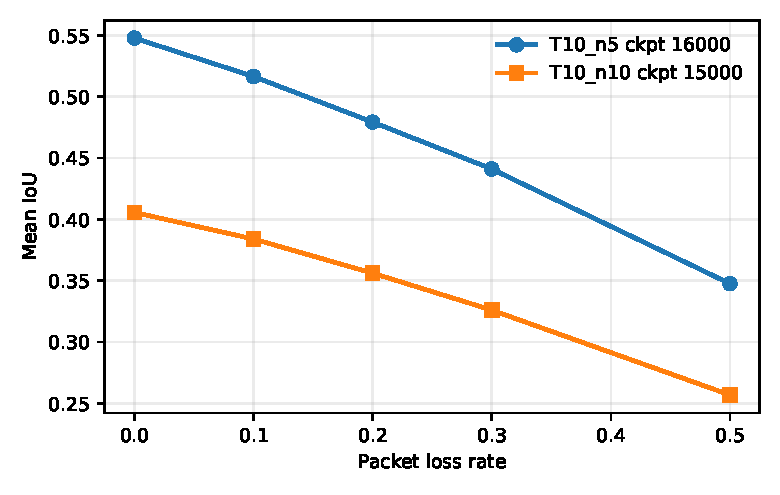
\includegraphics[width=0.95\linewidth]{pics/dair_packet_loss.pdf}
    \caption{DAIR-V2X-C VSPM robustness under packet loss. Performance degrades smoothly as packet loss increases, while the prediction model keeps positive gains over the copy-last-frame baseline in Table~\ref{tab:dair-robustness}.}
    \label{fig:dair-packet-loss}
\end{figure}

Finally, Table~\ref{tab:dair-robustness} and Fig.~\ref{fig:dair-packet-loss} evaluate robustness under packet loss, BEV dropout, and false positives. The mean IoU decreases as packet loss increases, which is expected because less historical information is available for stable prediction. Nevertheless, the IoU gain over the copy-last-frame baseline remains positive under all tested perturbations. This result indicates that DLPCM is not invariant to sensing and communication noise, but its degradation is gradual and remains explainable under realistic disturbances.

\section{Conclusion}
This work has demonstrated that both communication latency and computation latency exert a profound impact on the accuracy of cooperative perception, leading to severe safety risks in dynamic traffic environments. Beyond the widely acknowledged problem of communication latency, our study further proves that computation latency also plays a critical role in degrading perception accuracy. 
Through extensive evaluations on V2X-Sim and DAIR-V2X-C, we show that the proposed Dual-Latency Prediction Compensation Mechanism (DLPCM), together with the Vehicle-Specific Prediction Model (VSPM) and Model State Transmission (MST), achieves significant improvements in cooperative perception. The results demonstrate that our mechanism not only enhances real-time performance and prediction accuracy, but also alleviates communication pressure and reduces computational burden. The additional DAIR-V2X-C experiments further confirm the need for latency compensation in real cooperative perception and show that our VSPM and MST designs remain effective under real-scene BEV prediction, communication-state compression, and robustness evaluations. These findings validate the effectiveness and efficiency of the proposed framework in addressing the dual-latency challenge.
It is important to note that the emphasis of this work lies in the design of a new predictive compensation framework rather than the fine-tuning of specific prediction algorithms or compression strategies. While the framework already exhibits substantial advantages, future research will focus on improving the fidelity of prediction algorithms, exploring advanced compression methods for model state transmission, and conducting validations in large-scale heterogeneous cooperation. These directions will continue to strengthen the practicality of DLPCM and accelerate the safe and reliable deployment of cooperative perception in real-world intelligent driving systems.


















\bibliographystyle{IEEEtran}
\bibliography{ref.bib}




\newpage


 


\end{document}
